
%%%%%%%%%%%%%%%%%%%%%%%%%%%%%%%%%%%%%%%%%%%%%%%%%%%%%%%%%%%%%%%%%%%%%%%%
%
%		Chapter 1 - Mathematical Modelling
%
%%%%%%%%%%%%%%%%%%%%%%%%%%%%%%%%%%%%%%%%%%%%%%%%%%%%%%%%%%%%%%%%%%%%%%%%


\begin{topic}[Mathematical Modelling]
%\Title{Mathematical Modelling}

\label{chap1}
In this section, we study some strategies to model problems mathematically in an effective manner.

We also provide a structure to modelling problems by breaking them in small parts:

\begin{enumerate}[label={\bf \arabic*.}]
	\item \hyperref[moddefine]{Define the problem}
	\item \hyperref[mindmap]{Build a mind map}
	\item \hyperref[assumption]{Make assumptions}
%	\item \hyperref[D-parvsvar]{Decide on your parameters and variables}
	\item \hyperref[model]{Construct a model}
	\item \hyperref[analysis]{Analyze the model}
	\item \hyperref[report]{Write a report}
\end{enumerate}

\vspace{1cm}

In this chapter, we follow the approach of 
\begin{graybox}
\begin{minipage}{.8\textwidth}
\begin{verbatim}
	Math Modeling: Getting Started and Getting Solutions, K. M. Bliss, 
	K. R. Fowler, and B. J. Galluzzo, SIAM, Philadelphia, 2014
\end{verbatim}
\begin{center}
\url{https://m3challenge.siam.org/resources/modeling-handbook}
\end{center}
\end{minipage}
\hfill
\begin{minipage}{.17\textwidth}
	\hfill\qrcode{https://m3challenge.siam.org/resources/modeling-handbook}	
\end{minipage}
\end{graybox}
and
\begin{graybox}
\begin{minipage}{.8\textwidth}
\begin{verbatim}
	GAIMME: Guidelines for Assessment and Instruction in Mathematical
	Modeling Education, Second Edition, Sol Garfunkel and Michelle
	Montgomery, editors, COMAP and SIAM, Philadelphia, 2019
\end{verbatim}
\begin{center}
\url{http://uoft.me/gaimme}
\end{center}
\end{minipage}
\hfill
\begin{minipage}{.17\textwidth}
	\hfill\qrcode{http://uoft.me/gaimme}	
\end{minipage}
\end{graybox}


\vfill


\begin{center}
\begin{minipage}{300pt}
	\includegraphics*[width=300pt]{images/chap1-xkcd.jpg}

	\hfill {\footnotesize (image adapted from \href{https://www.xkcd.com/605/}{xkcd - comic \#605})}
\end{minipage}
\end{center}




\end{topic}






%%%%%%%%%%%%%%%%%%%%%%%%%%%%%%
%
%  MODULE - DEFINING THE PROBLEM
%
%%%%%%%%%%%%%%%%%%%%%%%%%%%%%%




\begin{module}{Defining the Problem}
	%\Title{Defining the Problem Statement}
	\label{moddefine}

		In this module you will learn
	\begin{itemize}
		\item how to define a problem mathematically.
	\end{itemize}

\hfill \\


The first step is to define the problem we want to solve.

\textbf{To do this, we should start from the end! }

We need to decide on what kind of mathematical object we will use in the end to show that we solved the problem we were tasked with. \\


Once this is done, we can define the problem mathematically. 

\begin{example}
	Your team was tasked with optimizing the layout of an airport. 

	The team decided to define:
	\begin{itemize}
		\item $T = $ the total time (in minutes) necessary by the average person to walk from their airport transportation (taxi, train, bus) to their gate, disregarding the time spent in security or immigration.
	\end{itemize}

	At the end of the project, to show that the team did find a good layout for the airport, the team will show that the new layout reduces the value of $T$. \\

	Once this decision is made, the problem to solve (or improve) becomes clear:
	
	\begin{itemize}
		\item Minimize $T$
	\end{itemize}

	There will probably be some constraints, which will be studied in Module \ref{assumption}.

\end{example}

	\begin{exercises}
		% Topics:
		% 
	For each exercise, what ``mathematical object'' would you use to communicate that you have solved or improved the problem? Then define the problem mathematically.
	\label{exercise:define}
	\begin{problist}
		% 
		\prob Help the city of Toronto choose the best recycling system.
		\prob Help the Canadian Institute of Health Information (CIHI) estimate how significant the outbreak of illnesses will be in the coming year in Canada.
		\prob Create a mathematical model to rank roller coasters according to thrill factor.
		\prob Gas stations offer different prices for gas. I would like to create an app that finds the best gas station to go to. What should ``best'' mean?
		\prob Is it better to buy or rent? 
		\begin{enumerate}
			\item Is it better to buy a car or rent Zipcar, or Car2go?
			\item Does the criteria you used to evaluate the previous question change if the question is whether to buy a bicycle or use Bike Share Toronto? 
		\end{enumerate}
		
		\prob Help Airbus design the interior of an airplane.
		
	\end{problist}
\end{exercises}

\end{module}


\begin{lesson}
	\Title{Defining Problem Statement}

	
\Heading{Textbook}
	\begin{itemize}
		\item Module 1
	\end{itemize}

\Heading{Objectives}
	\begin{itemize}
		\item The first step in Mathematical modelling is to define the problem
		\item A good way to do this is to figure out what is the ``mathematical object'' we are looking for at the end of the process

	\end{itemize}
	
\Heading{Motivation} 

\begin{annotation}
\begin{notes}
\begin{itemize}
	\item Students usually want to start thinking of ways to solve the problem.
	
	\item They need to learn to tackle a modelling task step-by-step.
\end{itemize}
\end{notes}	
\end{annotation}

Students have heard the words ``Model'' and ``Modelling'', yet they don't have a good idea what it means. 

The goal of this first chapter is to establish a common procedure to approach all  (or at least most) modelling tasks. 

The very first step in the procedure is to \emph{define the problem} in a clear and Mathematical way.

\Heading{Preparation for Class}
\begin{itemize}
	\item Read textbook
\end{itemize}


\Heading{Tutorials and Projects}
\begin{itemize}
	\item Project \ref{proj:erdos}: \erdostitle
	\item Project \ref{proj:elephants}: \elephantstitle
\end{itemize}

\begin{annotation}
	\vspace{-20pt}
	\begin{goals}
		\Goal{$\text{M}^{\text{2}} (\text{GS})^{\text{2}}$}
		\qrcode{https://m3challenge.siam.org/resources/modeling-handbook}
	\end{goals}
	\begin{goals}
		\Goal{GAIMME}
		\qrcode{http://uoft.me/gaimme}
	\end{goals}
\end{annotation}
	\Heading{Extra Reading} 
	
	\begin{itemize}
		\item \href{https://m3challenge.siam.org/resources/modeling-handbook}{Math Modelling: Getting started and getting solutions ($M^2(GS)^2$), Bliss-Fowler-Galluzzo -- pages 10-14} \\
		\hfill \url{https://m3challenge.siam.org/resources/modeling-handbook}
		
		\item \href{http://uoft.me/gaimme}{Guidelines for Assessment and Instruction in Mathematical Modeling Education (GAIMME), Garfunkel-Montgomery, editors}
		\hfill \url{http://uoft.me/gaimme}
	\end{itemize}
\end{lesson}






\def\email{
%	\thispagestyle{siam2019}
	\begin{graybox}
	-------- Forwarded Message -------- \\[10pt]
	\textbf{Date: } \dayofweekname{7}{9}{\the\year}, 7 September \the\year \; 21:41:35 + 0000  \\
	\textbf{From: } CEO <theCEO@theBigCompany.ca> \\
	\textbf{To: } Human Resources <hr@theBigCompany.ca> \\
	\textbf{Subject: } they're still late! \\
	
	Hey Shophika! \\
	
	I still get complaints about staff being late, some by 15 minutes.
	
	With the staff we have, that's about one salary lost.
	
	Again the bottleneck of the elevators seems to be the problem.
	
	Can you suggest solutions? \\
	
	Thanks, the CEO
	\end{graybox}
	
	(\newurl{problem adapted from GAIMME, SIAM}{http://uoft.me/gaimme})
}

%Elevator problem at theBigCompany

%\addcontentsline{toc}{subsection}{Task 1.A: Elevator problem at theBigCompany}

\begin{annotation}
	\begin{goals}
		\Goal{Make the question precise, bring it into a ``mathematical form''.}
		\begin{itemize}
			\item Choose a mathematical object best suited for the problem, e.g. a number, a geometric form, a graph, a function, an algorithm, ...

		\end{itemize}
	\end{goals}
%	\begin{notes}
%		
%		\begin{itemize}
%			\item There are many ways to solve this problem.
%				Some students
%				might start with equations. After they use their
%				equations to solve the problem, make them draw a picture
%				and come up with a graphical solution.
%
%			\item When the students start coming up with vector equations,
%				give them the vocabulary of \emph{linear
%				combinations}
%				and \emph{column vector notation}.
%		\end{itemize}
%	\end{notes}
	\begin{notes}
		
		\begin{itemize}
			\item Students will start discussing how to solve the problem
			\item This question deals with what will happen \textbf{after} solving the problem
			\item The goal of this question is to think about how to best tell a ``mathematically-challenged'' CEO that you solved the problem
			\item Student teamwork: ``With your team, you must decide on one answer and be prepared to report on your decision and the reason for your choice.''
		\end{itemize}
	\end{notes}
\end{annotation}

\question \label{elevator-define}
You are hired by theBigCompany to help with their ``elevator problem''.

This is the email you received:

\begin{center}
\begin{minipage}{.75\textwidth}
	\email
\end{minipage}
\end{center}


%\vspace{5mm}

What mathematical object would you use to convince the CEO that you have solved or improved the problem? 


\begin{teamwork}
	With your team, you must decide on \emph{one} answer and be prepared to report on your decision and the reason for your choice.	
\end{teamwork}

\bookonlynewpage







\question 

The mayor of Toronto wants to extend the subway line with a new \textbf{\color{orange}orange line} as in the figure below. \label{p:TTC}
	
%	\begin{center}
%	\includegraphics*[width=500pt]{images/TTC-extension.png}
%	\end{center}

\begin{center}
	\includegraphics*[width=500pt]{images/TTC.png}
\end{center}
\begin{minipage}{1.1\textwidth}
\hfill {\footnotesize (Map taken from \href{https://uoft.me/modelling-TTC}{Wikimedia Commons} created by Craftwerker) \qquad \qrcode[height=30pt]{https://uoft.me/modelling-TTC}}
\end{minipage}
	
\begin{parts}
	\item What ``mathematical object'' would you use to communicate that to the Mayor that this line is optimal (or sub optimal) ?

	\item Define the problem mathematically.
\end{parts}
















\standardonlynewpage


%%%%%%%%%%%%%%%%%%%%%%%%%%%%%%
%
%  MODULE - Mind Map
%
%%%%%%%%%%%%%%%%%%%%%%%%%%%%%%



\begin{module}{Building a mind map}
	%\Title{Building a mind map}
	\label{mindmap}

	\begin{siam}
	
	In this module you will learn
	\begin{itemize}
		\item How to create a mindmap.
	\end{itemize}


\hfill \\



%\Heading{Mind Map}

A mind map is a tool to visually outline and organize ideas. Typically a key idea is the centre of a mind map and associated ideas are added to create a diagram that shows the flow of ideas. 

\begin{example}\label{ex-recycling}

Let us focus on the question: ``What is the best recycling system for Toronto?''

Then we can think of many different definitions for what the word ``best'' means:

\begin{itemize}
	\item The system that gets the most participation from the population, which can be measured by the fraction of the Toronto households participating in recycling;
	\item The system that costs the least amount of money for the city. How can this be measured?
	\item The system that processes the most amount of recyclables.
\end{itemize}

In the figure below, we focus on the definition of ``best'', with these three possible definitions branching off to be further explored.

\def\MindMapOne{
	\fill[color=lime] (0,0) rectangle (4,1) node[pos=.5] {\color{black}``Best'' recycling centre};
	\fill[color=BurntOrange] (6,2.5) rectangle (8,1.5) node[pos=.5] {\color{black}\begin{minipage}{40pt}\raggedright Most participation\end{minipage}};
	\fill[color=Goldenrod] (6,0) rectangle (8,1) node[pos=.5] {\color{black}\begin{minipage}{45pt}\raggedright Least cost to the city\end{minipage}};
	\fill[color=red!70!white] (6,-2) rectangle (8,-0.5) node[pos=.5] {\color{black}\begin{minipage}{50pt}\raggedright Processes the most recyclables\end{minipage}};
	\draw (4,0.75) -- (6,2);
	\draw (4,0.5) -- (6,0.5);
	\draw (4,0.25) -- (6,-1.25);
%
%	\fill[color=Green!60!white] (0,0) rectangle (4,1) node[pos=.5] {\color{black}``Best'' recycling centre};
%	\fill[color=BurntOrange] (7,2.5) rectangle (11,1.5) node[pos=.5] {\color{black}Most participation};
%	\fill[color=Goldenrod] (7,0) rectangle (11,1) node[pos=.5] {\color{black}Least cost to the city};
%	\fill[color=red] (7,-1.5) rectangle (12,-0.5) node[pos=.5] {\color{black}Processes the most recyclables};
%	\draw (4,0.75) -- (7,2);
%	\draw (4,0.5) -- (7,0.5);
%	\draw (4,0.25) -- (7,-1);
}

\begin{center}
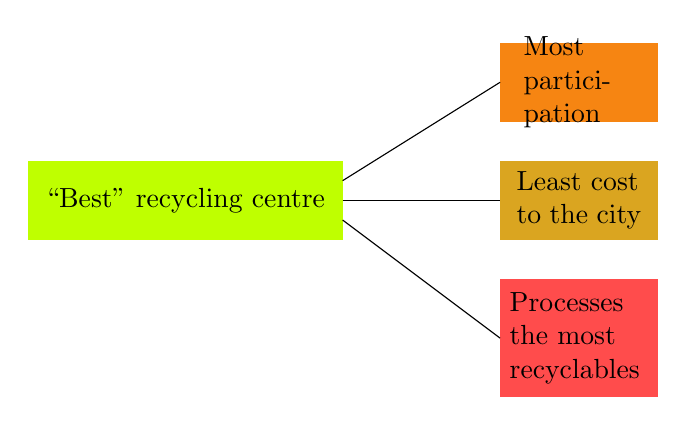
\begin{tikzpicture}
\MindMapOne
%	\fill[color=lime] (0,0) rectangle (4,1) node[pos=.5] {\color{black}``Best'' recycling centre};
%	\fill[color=BurntOrange] (7,2.5) rectangle (11,1.5) node[pos=.5] {\color{black}Most participation};
%	\fill[color=Goldenrod] (7,0) rectangle (11,1) node[pos=.5] {\color{black}Least cost to the city};
%	\fill[color=red] (7,-1.5) rectangle (12,-0.5) node[pos=.5] {\color{black}Processes the most recyclables};
%	\draw (4,0.75) -- (7,2);
%	\draw (4,0.5) -- (7,0.5);
%	\draw (4,0.25) -- (7,-1);
\end{tikzpicture}
\end{center}

%\end{example}


%\begin{figure}[!ht]
%\begin{tikzpicture}
%	\fill[color=Green] (0,0) rectangle (4,1) node[pos=.5] {\color{black}``Best'' recycling centre};
%	\fill[color=BurntOrange] (7,2.5) rectangle (11,1.5) node[pos=.5] {\color{black}Most participation};
%	\fill[color=Goldenrod] (7,0) rectangle (11,1) node[pos=.5] {\color{black}Least cost to the city};
%	\fill[color=red] (7,-1.5) rectangle (12,-0.5) node[pos=.5] {\color{black}Processes the most recyclables};
%	\draw (4,0.75) -- (7,2);
%	\draw (4,0.5) -- (7,0.5);
%	\draw (4,0.25) -- (7,-1);
%\end{tikzpicture}
%\caption{An example of a simple mind map.}
%\label{mindmap1}
%\end{figure}

 From here, we can focus our attention on one of the branches at a time. \\



%\begin{example}

Let's think about the least-cost option first. 

We probably can't determine how much any recycling program costs without knowing more about the recycling program, so a good place to start is to ask the question ``What kinds of recycling programs exist?''

If we aren't familiar with different types of recycling, we might need to do some research to see what kinds of programs exist.

A possible next step on your mind map for the least-cost approach could be the one shown below. %in Figure \ref{mindmap2}.


\begin{center}
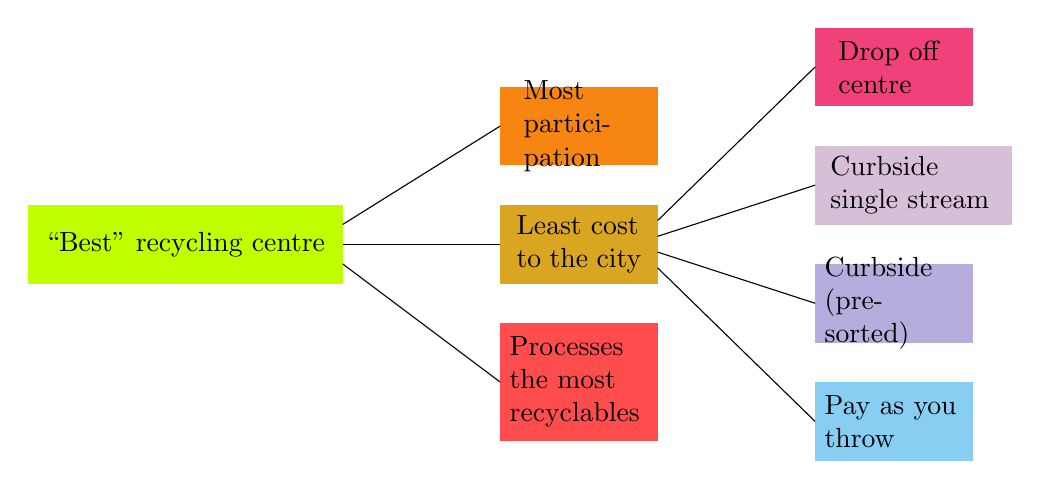
\begin{tikzpicture}
\MindMapOne
%	\fill[color=lime] (0,0) rectangle (4,1) node[pos=.5] {\color{black}``Best'' recycling centre};
%	\fill[color=BurntOrange] (6,2.5) rectangle (8,1.5) node[pos=.5] {\color{black}\begin{minipage}{40pt}\raggedright Most participation\end{minipage}};
%	\fill[color=Goldenrod] (6,0) rectangle (8,1) node[pos=.5] {\color{black}\begin{minipage}{45pt}\raggedright Least cost to the city\end{minipage}};
%	\fill[color=red] (6,-2) rectangle (8,-0.5) node[pos=.5] {\color{black}\begin{minipage}{50pt}\raggedright Processes the most recyclables\end{minipage}};
%	\draw (4,0.75) -- (6,2);
%	\draw (4,0.5) -- (6,0.5);
%	\draw (4,0.25) -- (6,-1.25);
	\fill[color=WildStrawberry!80!white] (10,2.25) rectangle (12,3.25) node[pos=.5] {\color{black}\begin{minipage}{40pt}\raggedright Drop off centre\end{minipage}};	
	\fill[color=Thistle] (10,0.75) rectangle (12.5,1.75) node[pos=.5] {\color{black}\begin{minipage}{60pt}\raggedright Curbside single stream\end{minipage}};	
	\fill[color=Periwinkle!50!white] (10,0.25) rectangle (12,-0.75) node[pos=.5] {\color{black}\begin{minipage}{50pt}\raggedright Curbside (pre-sorted)\end{minipage}};	
	\fill[color=Cerulean!50!white] (10,-2.25) rectangle (12,-1.25) node[pos=.5] {\color{black}\begin{minipage}{50pt}\raggedright Pay as you throw\end{minipage}};
	\draw (8,0.8) -- (10,2.75);	
	\draw (8,0.6) -- (10,1.25);	
	\draw (8,0.4) -- (10,-0.25);	
	\draw (8,0.2) -- (10,-1.75);	
\end{tikzpicture}
\end{center}
\end{example}
\end{siam}

%\begin{figure}[!htbp]
%\begin{tikzpicture}
%	\fill[color=Green] (0,0) rectangle (4,1) node[pos=.5] {\color{black}``Best'' recycling centre};
%	\fill[color=BurntOrange] (6,2.5) rectangle (8,1.5) node[pos=.5] {\color{black}\begin{minipage}{40pt}\raggedright Most participation\end{minipage}};
%	\fill[color=Goldenrod] (6,0) rectangle (8,1) node[pos=.5] {\color{black}\begin{minipage}{45pt}\raggedright Least cost to the city\end{minipage}};
%	\fill[color=red] (6,-2) rectangle (8,-0.5) node[pos=.5] {\color{black}\begin{minipage}{50pt}\raggedright Processes the most recyclables\end{minipage}};
%	\draw (4,0.75) -- (6,2);
%	\draw (4,0.5) -- (6,0.5);
%	\draw (4,0.25) -- (6,-1.25);
%	\fill[color=WildStrawberry] (10,2.25) rectangle (12,3.25) node[pos=.5] {\color{black}\begin{minipage}{40pt}\raggedright Drop off centre\end{minipage}};	
%	\fill[color=Thistle] (10,0.75) rectangle (12.5,1.75) node[pos=.5] {\color{black}\begin{minipage}{60pt}\raggedright Curbside single stream\end{minipage}};	
%	\fill[color=Periwinkle] (10,0.25) rectangle (12,-0.75) node[pos=.5] {\color{black}\begin{minipage}{50pt}\raggedright Curbside (pre-sorted)\end{minipage}};	
%	\fill[color=Cerulean] (10,-2.25) rectangle (12,-1.25) node[pos=.5] {\color{black}\begin{minipage}{50pt}\raggedright Pay as you throw\end{minipage}};
%	\draw (8,0.8) -- (10,2.75);	
%	\draw (8,0.6) -- (10,1.25);	
%	\draw (8,0.4) -- (10,-0.25);	
%	\draw (8,0.2) -- (10,-1.75);	
%\end{tikzpicture}
%\caption{Next step of a mind map.}
%\label{mindmap2}
%\end{figure}


\begin{important}
		There is free online software to help creating a mind map. One such is \href{http://freemind.sourceforge.net}{FreeMind (http://freemind.sourceforge.net)}.
		
		\hfill \qrcode{http://freemind.sourceforge.net}
\end{important}


\begin{graybox}
\begin{minipage}{.75\textwidth}
For more details on creating a mind map, check the book:
\begin{verbatim}
	Math Modeling: Getting Started and Getting Solutions, K. M. Bliss, K. R. Fowler, 
	and B. J. Galluzzo, SIAM, Philadelphia, 2014
\end{verbatim}
\begin{center}
\href{https://m3challenge.siam.org/resources/modeling-handbook}{\tt https://m3challenge.siam.org/resources/modeling-handbook}
\end{center}
\end{minipage}
\hfill
\begin{minipage}{.20\textwidth}
	\hfill\qrcode{https://m3challenge.siam.org/resources/modeling-handbook}	
\end{minipage}
\end{graybox}






	\begin{exercises}
		% Topics:
		% 
	\begin{problist}
		% 
		\prob
		Expand the mind map from the example above by focusing on the other two approaches:
		\begin{enumerate}
			\item Most participation
			\item Processes the most recyclables
		\end{enumerate}

		
	For each part, create a mind map. 
	Focus on the same approach you had for the \hyperref[exercise:define]{questions from the previous module}.

		\prob Help the Canadian Institute of Health Information (CIHI) estimate how significant the outbreak of illnesses will be in the coming year in Canada.
		\prob Create a mathematical model to rank roller coasters according to thrill factor.
		\prob Gas stations offer different prices for gas. I would like to create an app that finds the best gas station to go to. What should ``best'' mean?
		\prob The mayor of Toronto wants to extend the subway line with a new orange line as in \hyperref[p:TTC]{core exercise \ref{p:TTC}}. Is it optimal?
		
		\prob Is it better to buy a car or rent Zipcar, or Car2go?
		
		\prob Help Airbus design the interior of an airplane.

	\end{problist}
\end{exercises}

\end{module}



\begin{lesson}
	\Title{Building a mind map}


\Heading{Textbook}
	\begin{itemize}
		\item Module 2
	\end{itemize}

\Heading{Objectives}
	\begin{itemize}
%		\item The second step is to create a mind map of the problem. This is a structured way to brainstorm possible solutions, their requirements, and other objects that affect or are affected.

		\item The second step in Mathematical modelling is to construct a representation of how the team will be attempting to solve the problem.

		\item Create a mind map of the problem. This is a structured way to brainstorm possible solutions, requirements, other objects that are related, etc.
	\end{itemize}
	
\Heading{Motivation} 

In this step, students are supposed to brainstorm and relate the problem at hand with everything that is affected or can be affected by it.

The idea is to get a simple visual representation of possible solutions, without all the details. \\

This is a fundamental step in modelling.


\Heading{Preparation for Class}
\begin{itemize}
	\item Read textbook
\end{itemize}


\Heading{Tutorials and Projects}
\begin{itemize}
	\item Project \ref{proj:dragons}: \dragonstitle
	\item Project \ref{proj:erdos}: \erdostitle
	\item Project \ref{proj:elephants}: \elephantstitle
\end{itemize}


\begin{annotation}
	\vspace{-20pt}
	\begin{goals}
		\Goal{$\text{M}^{\text{2}} (\text{GS})^{\text{2}}$}
		\qrcode{https://m3challenge.siam.org/resources/modeling-handbook}
	\end{goals}
	\begin{goals}
		\Goal{GAIMME}
		\qrcode{http://uoft.me/gaimme}
	\end{goals}
\end{annotation}
	\Heading{Extra Reading} 
	
	\begin{itemize}
		\item \href{https://m3challenge.siam.org/resources/modeling-handbook}{Math Modelling: Getting started and getting solutions ($M^2(GS)^2$), Bliss-Fowler-Galluzzo -- pages 10-14} \\
		\hfill \url{https://m3challenge.siam.org/resources/modeling-handbook}
		
		\item \href{http://uoft.me/gaimme}{Guidelines for Assessment and Instruction in Mathematical Modeling Education (GAIMME), Garfunkel-Montgomery, editors}
		\hfill \url{http://uoft.me/gaimme}
	\end{itemize}
\end{lesson}




%\newpage


\question
\label{elevatorR}
Consider the elevator problem from question \ref{elevator-define}.


\begin{annotation}
	\begin{notes}
	\begin{itemize}
		\item Students usually come up with more complicated variations:
		\begin{itemize}
			\item Money spent on late employees' salaries
			\item sum of time in minutes that employees are late counting only employees that are at most 15 minutes late
		\end{itemize}
		\item Stick with $T$, a simple first approach
	\end{itemize}	
	\end{notes}
	
\end{annotation}
Your team decides that the mathematical object you will use to show the CEO that you solved or improved the problem is
\begin{itemize}
	\item $T=$ the sum in minutes by which every employee is late.
\end{itemize}

Note that employees that are on time count for 0 minutes (not a negative amount of minutes). \\

Create a mind map for the question: \quad How can $T$ be minimized?


\bookonlynewpage


\question

The city of Toronto decided to tear down the Gardiner expressway. While the demolition is taking place, several key arteries are closed and many intersections are bottled. 
At peak times, a police officer is often posted at this intersection to \emph{optimally} control the traffic lights. 

\begin{parts}
	\item What mathematical meaning can we give to the word optimal in this circumstance? 
	\item Create a mind map for this problem.
\end{parts}




	









\standardonlynewpage


%%%%%%%%%%%%%%%%%%%%%%%%%%%%%%
%
%  MODULE - Making Assumptions
%
%%%%%%%%%%%%%%%%%%%%%%%%%%%%%%



\begin{module}{Making assumptions}
	%\Title{Making Assumptions}
	\label{assumption}

\begin{siam}
	In this module you will learn
\begin{itemize}
	\item that we need to make assumptions to be able to create a model
	\item how to strike a balance between accuracy and solvability
\end{itemize}

\hfill \\




Real problems are complex, so when modelling a real problem mathematically, we must make some assumptions. 

The assumptions that we make will affect the problem we are solving and its difficulty, so we need to strike a balance between:
\begin{itemize}
\item accuracy -- the fewer assumption the better, and
\item solvability -- the more assumptions the better.
\end{itemize}

\begin{annotation}
	\begin{goals}
		When building a mind map, keep track of the assumptions necessary for each step.
	\end{goals}
\end{annotation}

Many assumptions follow naturally when building a mind map. \\


\begin{annotation}
	\begin{goals}
		Remember to justify all your assumptions.
	\end{goals}
\end{annotation}

When figuring which assumption to make, keep in mind the key-factors of the problem and find data when available (usually online). 
If not available, measure data when possible, and if it's not possible, make a reasonable assumption on what the data might look like.

Another thing to keep in mind are \emph{time constraints}. Whether in a class, test, or working in a project, there will be deadlines. Your assumptions should take time constraints into consideration. 



\begin{example}

AN EXAMPLE, PROBABLY BASED ON THE RECYCLING.
	
\end{example}




%\hfill \\

%	\section*{Step D. Parameters or Variables?}\label{D-parvsvar}
%	\addcontentsline{toc}{subsection}{Step D. Parameters or Variables?}
%	
%	
%	
%	When you have defined the problem you want to solve and you have made your (initial) assumptions, it is then time to define some details of the problem.
%	
%	
%	
%	
%	With the problem statement clearly defined and an initial set of assumptions made (a list that will likely get longer), you are ready to start to define the details of your model. Now is the time to pause to ask what
%	is important that you can measure. Identifying these notions as variables, with units and some sense of their range, is key to building the model.
%	The purpose of a model is to predict or quantify something of interest. We refer to these predictions
%	as the outputs of the model. Another term we use
%	for outputs is dependent variables. We will also have independent variables, or inputs to the model. Some quantities in a model might be held constant, in which case they are referred to as model parameters. Let's look at a few simple examples that will help you distinguish between these concepts. We'll also see how they depend on your viewpoint and the problem statement.
%	
%	
%	
%	%There is a clear difference between \emph{variables} and \emph{parameters}. 
%	
%	\begin{definition}[Variables and Parameters]
%	
%	
%	A \emph{variable} represents a model state, and may change during simulation.
%	
%	A \emph{parameter} is commonly used to describe objects statically. A \emph{parameter} is normally a constant in a single simulation, and is changed only when you need to adjust your model behaviour. 
%	\end{definition}
%	
%	%Use a variable instead of a parameter if you need to model some data unit continuously changing over time. Use a parameter instead of a variable if you just need to model some parameter of an object changed only at particular moments of time.
%	
%	
%	
%	\begin{annotation}
%		\begin{goals}
%		\qrcode{https://en.wikipedia.org/wiki/Parameter\#Mathematical\_models}	
%		\end{goals}
%	\end{annotation}
%	\begin{note}{(from Wikipedia)}
%	The quantities appearing in the equations we classify into variables and parameters. The distinction between these is not always clear cut, and it frequently depends on the context in which the variables appear. 
%	
%	Usually a model is designed to explain the relationships that exist among quantities which can be measured independently in an experiment; these are the \emph{variables} of the model. 
%	
%	To formulate these relationships, however, one frequently introduces ``constants'' which stand for inherent properties of nature (or of the materials and equipment used in a given experiment). These are the \emph{parameters}.	
%	\end{note}






%
%
%
%The choice of question in the previous module should determine the \emph{dependent} variable.

%
%The \emph{parameters} are the independent variables in the problem, e.g. the speed of the elevators. The final answer will depend on the parameters in the problem. 
%
%We can estimate the parameters, and sometimes even change them. \\
%
%The \emph{variables} are dependent. This meant that if we change the parameters, the variables will change automatically. 

	\begin{exercises}
		% Topics:
		% 
	\begin{problist}
	\prob
	For each part, you are required to make an estimate for some quantity. Make assumptions and justify them in order to solve the problem.
		\begin{enumerate}
			\item What is the number of piano players in Toronto? \hfill \emph{(Fermi problem)}
			\item How many linear km of roads are there in Toronto?
			\item How much salt the city of Toronto needs for its roads during the Winter?
			\item The skating season in Canada is shortening: What are the key-factors determining its length?
		\end{enumerate}
	\end{problist}
\end{exercises}

\end{siam}
\end{module}
	



\begin{lesson}
	\Title{Making Assumptions}

\Heading{Textbook} 
	\begin{itemize}
		\item Module 3
	\end{itemize}

\Heading{Objectives}
	\begin{itemize}
		\item The third step is to decide on a path to the solution and start making assumptions.
		
		\item This is a difficult balance between:
		\begin{itemize}
			\item Accuracy, but difficult to analyze/solve;
			\item Simple, easy to analyze/solve but not very accurate.
		\end{itemize}

	\item Make sure assumptions and conditions of the modelling are clearly mentioned to the future reader/user of the model
	\end{itemize}
	
	
\Heading{Motivation} 

Students often make assumptions explicitly and implicitly, but they often keep them out of their notes. In the end they forget to include them in the final report.

\begin{annotation}
\begin{goals}
	\Goal{Assumptions.}
	Include the assumptions in the model's final report.
\end{goals}
\end{annotation}
It is imperative that they include their assumptions in the final report of their model.

Moreover, students should make an effort to find out the implicit assumptions and the conditions that to the model that their assumptions require.


\Heading{Preparation for Class}
\begin{itemize}
	\item Read textbook
\end{itemize}

\Heading{Tutorials and Projects}
\begin{itemize}
	\item Project \ref{proj:dragons}: \dragonstitle
	\item Project \ref{proj:erdos}: \erdostitle
	\item Project \ref{proj:elephants}: \elephantstitle
\end{itemize}

\begin{annotation}
	\vspace{-20pt}
	\begin{goals}
		\Goal{$\text{M}^{\text{2}} (\text{GS})^{\text{2}}$}
		\qrcode{https://m3challenge.siam.org/resources/modeling-handbook}
	\end{goals}
	\begin{goals}
		\Goal{GAIMME}
		\qrcode{http://uoft.me/gaimme}
	\end{goals}
\end{annotation}
	\Heading{Extra Reading} 
	
	\begin{itemize}
		\item \href{https://m3challenge.siam.org/resources/modeling-handbook}{Math Modelling: Getting started and getting solutions ($M^2(GS)^2$), Bliss-Fowler-Galluzzo -- pages 15-19} \\
		\hfill \url{https://m3challenge.siam.org/resources/modeling-handbook}
		
		\item \href{http://uoft.me/gaimme}{Guidelines for Assessment and Instruction in Mathematical Modeling Education (GAIMME), Garfunkel-Montgomery, editors}
		\hfill \url{http://uoft.me/gaimme}
	\end{itemize}
\end{lesson}




%\newpage

\begin{minipage}{.5\textwidth}	
\question
\label{elevator-assumptions}
Consider the elevator problem from \hyperref[elevator-define]{core exercise \ref{elevator-define}}. 


We now give you some technical details about \nobreak{theBigCompany}:

\begin{itemize}
	\item The company occupies the floors 30--33 of the building Place Ville-Marie in Montr\'eal.

	\item Personnel is distributed in the following way: 
	\begin{itemize}
		\item 350 employees in floor 30,
		\item 350 employees in floor 31,
		\item 250 employees in floor 32, 
		\item 150 employees in floor 33.
	\end{itemize}
\end{itemize}

\emph{Note.} Even though these details are fictional, the numbers respect the building code. \\

\emph{Hint.} Focus on a \textbf{few} parameters and variables.
\end{minipage}
\qquad
\begin{minipage}{.5\textwidth}	
\email
\end{minipage}

\begin{annotation}
	\begin{notes}
		\begin{itemize}
			\item Students usually have trouble starting. 
			\item They usually agree that they have to figure out how elevators work, so you can prompt them to be more specific. 
			
			\item In the end they should come up with questions like these:
			\begin{itemize}
				\item How fast are the elevators?
				\item How much time do elevators take in each floor?
				\item How many floors do elevators stop on their way up?
				\item How many people fit in the elevator?
				\item Should we consider elevator failures?
			\end{itemize}
		\end{itemize}	
	\end{notes}
\end{annotation}
\begin{parts} 
	\item With your team, decide on what kind of information you would need to have to be able to solve this problem.

	\item Find the relevant information about the elevators (search the internet, by experimentation). Check the reliability of the data you found.

	\item For the relevant information that you cannot obtain, make assumptions. These assumptions should be reasonable and you should be able to justify them.
\end{parts}




\bookonlynewpage

\begin{notslides}

\hfill

\bookonlynewpage
\end{notslides}

\question How much would it cost to make a bridge between Toronto and the U.S.?














\standardonlynewpage

%%%%%%%%%%%%%%%%%%%%%%%%%%%%%%
%
%  MODULE - Construction of the Model
%
%%%%%%%%%%%%%%%%%%%%%%%%%%%%%%



\begin{module}{Construct a model}
%	\Title{Construct a model}
	\label{model}

\begin{siam}

In this module you will learn
\begin{itemize}
	\item how to build a model based on the previous steps
\end{itemize}

\hfill

	
In this module you will learn
\begin{itemize}
	\item how to build a model based on the previous steps
\end{itemize}

\hfill \\



This is the part of the modelling where we connect all that we have done so far: the problem we defined, the mind map, the assumptions, and all the variables and parameters in a mathematical model to answer the ``mathematical'' problem defined in \hyperref[define]{Step A}.


%When you have defined the problem you want to solve and you have made your (initial) assumptions, it is then time to define some details of the problem.
	
	
With the problem statement clearly defined and an initial set of assumptions made (a list that will likely get longer), you are ready to start to define the details of your model. Now is the time to pause to ask what is important that you can measure. 
Identifying these notions as variables, with units and some sense of their range, is key to building the model.

The purpose of a model is to predict or quantify something of interest. %We refer to these predictions as the outputs of the model. 
	
Creating a model usually means writing down mathematical equations, constructing a graph, analyzing a geometric figure, or do some statistical analysis. \\


\begin{example}
Your team is tasked with finding the best recycling centre (we looked at this example in \hyperref[mindmap]{Step B}) and your  team has chosen to minimize the cost to the city by using drop off centres.

As part of modelling process, your team has made the following assumptions/measurements:
\begin{itemize}
	\item People would be willing to pay \$2.29 to recycle per month or \$0.53 per week
	\item People would make one weekly trip to the centre
	\item Gasoline costs around \$1.26 per litre
	\item On average a passenger car consumes 10 litres per hundred kilometres\\
\end{itemize}

This means that the (one-way) distance people are willing to travel every week to the drop-off centre is
$$
d \;=\; \frac{1}{4.3 \text{ trips/month}} \cdot \frac{\$2.29 / {\text{month}} }{(\$1.26 \text{/L}) \ \cdot\  (0.1 \text{ L / km})} \;=\; 4.2 \text{  km/trip}.
$$

This should help us figure out the best way to place the drop-off centres. \\

The Mathematical model might look like this

\begin{itemize}
	\item Maximize (number of people within a 4.2 km radius of a drop-off centre)
	\item subject to a certain number of drop-off centres (given by the city budget) %\\
\end{itemize}

%\textit{Note. } The model should also include the cost of building a drop off centre.
\end{example}

\begin{graybox}
Assuming that this project was requested for a specific city, the final report should also include some suggested locations for various different budgets.	
\end{graybox}


%\hfill
%
%Sometimes, the mathematical tools necessary to tackle the problem are clear, but often they are not. In those cases it may be helpful to analyze some simple cases.




	\begin{exercises}
		% Topics:
		% 
	\begin{problist}
	\prob
	For each part, create a model to answer the question. Remember all the previous steps.

	\begin{enumerate}
	\item You want to open a piano store in Toronto, where should you open it?
	\item There was a big snow storm in Toronto and the roads need cleaning. How should the city deploy its snow plowers?
	\item The city of Toronto wants to deactivate the Pickering nuclear power plant in favour of renewable power sources. What is the best way to create the same amount of electricity using only renewable sources in the GTA?
	\item Loblaws wants to start an online food delivery service. How should they do it?
	\item The city airport (YTZ) built a tunnel to access the island airport from the city. Before that, they used a ferry. Was building the tunnel a good decision?	
		\end{enumerate}
	\end{problist}
\end{exercises}

\end{siam}

\end{module}



\begin{lesson}
	\Title{Construct a model}

\Heading{Textbook} 
	\begin{itemize}
		\item Module 4
	\end{itemize}

\Heading{Objectives}
	\begin{itemize}
		\item The fourth step is to use the mind map created in step 2, the assumptions from step 3, and assemble everything into one model.
		
		\item The model is not the solution to the problem: it is the framework to solve the problem. 
	\end{itemize}
	

\Heading{Motivation} 

\begin{annotation}
\begin{notes}
	\begin{itemize}
	\item Model $\neq$ Solution
	\end{itemize}
\end{notes}
\end{annotation}
Students usually think that the solution is the model that they need.

Emphasize that students should see the example in the textbook to get an idea of what a model looks like.

\begin{annotation}
\begin{notes}
	There won't be enough time in class to finish the question if students don't prepare in advance.
\end{notes}	
\end{annotation}

\Heading{Preparation for Class}
\begin{itemize}
	\item Read textbook
	\item Ask students to prepare the core exercise \ref{model:preclass} before class.

	\item In class, they should combine their mind map(s) and assumptions from the previous lessons and come up with an idea of a model to discuss with their classmates in lecture.

\end{itemize}

\Heading{Tutorials and Projects}
\begin{itemize}
	\item Project \ref{proj:dragons}: \dragonstitle
	\item Project \ref{proj:erdos}: \erdostitle
	\item Project \ref{proj:elephants}: \elephantstitle
\end{itemize}


\begin{annotation}
	\vspace{-20pt}
	\begin{goals}
		\Goal{$\text{M}^{\text{2}} (\text{GS})^{\text{2}}$}
		\qrcode{https://m3challenge.siam.org/resources/modeling-handbook}
	\end{goals}
	\begin{goals}
		\Goal{GAIMME}
		\qrcode{http://uoft.me/gaimme}
	\end{goals}
\end{annotation}
	\Heading{Extra Reading} 
	
	\begin{itemize}
		\item \href{https://m3challenge.siam.org/resources/modeling-handbook}{Math Modelling: Getting started and getting solutions ($M^2(GS)^2$), Bliss-Fowler-Galluzzo -- pages 20-31} \\
		\hfill \url{https://m3challenge.siam.org/resources/modeling-handbook}
		
		\item \href{http://uoft.me/gaimme}{Guidelines for Assessment and Instruction in Mathematical Modeling Education (GAIMME), Garfunkel-Montgomery, editors}
		\hfill \url{http://uoft.me/gaimme}
	\end{itemize}
\end{lesson}




%\newpage



\begin{minipage}{.5\textwidth}	
\question \label{model:preclass}
Recall the \hyperref[elevator-assumptions]{core exercise \ref{elevator-assumptions}}.

\begin{itemize}
	\item The company occupies the floors 30--33 of the building Place Ville-Marie in Montr\'eal.

	\item Personnel is distributed in the following way: 
	\begin{itemize}
		\item 350 employees in floor 30,
		\item 350 employees in floor 31,
		\item 250 employees in floor 32, 
		\item 150 employees in floor 33.
	\end{itemize}
\end{itemize}

%\vspace{1 .5cm}

Write down a mathematical model for this problem.
\label{elevator-model}

\begin{teamwork}
Each team should have \emph{one} model and be prepared to present it to the class.	
\end{teamwork}

\end{minipage}
\qquad
\begin{minipage}{.5\textwidth}	
\email
\end{minipage}

\begin{annotation}
\begin{goals}
	\Goal{Create a model.}
	\begin{enumerate}[label=\textbf{\color{Cerulean}\arabic*.}]
		\item Students should join in teams of 2--4 and come up with \emph{one model} for the team.
		\item The model should include:
		\begin{itemize}
			\item Definition of the problem
			\item Mind map
			\item Assumptions and conditions
			\item Clearly defined path to solve the problem
		\end{itemize}
		\item A few teams present their model for everyone else.
		\item Full class brainstorm about each model:
		\begin{itemize}
			\item Does it include all the parts specified?
			\item Is it solvable? 
			\item Could we make some extra assumptions to make it simpler?
			\item Is it accurate?
			\item Could we change something to make it more accurate without sacrificing simplicity?
		\end{itemize}
	\end{enumerate}
\end{goals}	
\begin{notes}
Suggestions to help students get started:
\begin{itemize}
	\item How long do all employees take to get to work?
	\item When do they arrive to the building?
	\item First: evaluate the situation -- don't try to fix the problem
\end{itemize}	
\end{notes}
\end{annotation}


















\standardonlynewpage


%%%%%%%%%%%%%%%%%%%%%%%%%%%%%%
%
%  MODULE - Model Assessment
%
%%%%%%%%%%%%%%%%%%%%%%%%%%%%%%



\begin{module}{Model Assessment}
	%\Title{Model Assessment}
	\label{analysis}

\begin{siam}
	
In this module you will learn
\begin{itemize}
	\item how to analyze a model
	\item to check the quality of the model
\end{itemize}

\hfill \\



At this point, you have defined a problem statement, and a mind map to help you decide how to approach the problem. You have made assumptions and made note of them and justified them.
You finally created a model to solve the problem.

The next step is to analyze the model.

There are two types of analysis:


\paragraph{\textcolor{cyan}{\textbf{Superficial assessment.}}} Are the units correct? Are the variables and parameters of a reasonable magnitude? Does it behave as expected? Does it make sense?



\paragraph{\textcolor{cyan}{\textbf{In-depth assessment.}}} Once the superficial assessment is verified, we need to understand the model at a deeper level. 

What are the model's strengths? What are its weaknesses?

When you change the inputs of the model, how do the outputs change? This is called {\emph sensitivity analysis}. 


%Next is a simple example adapted from \cite{bliss}.


%\begin{annotation}
%	\begin{goals}
%	\Goal{Desmos Graph}
%	\hfill \qrvideo{https://www.desmos.com/calculator/z9cftzus0z}
%	\end{goals}
%\end{annotation}

\begin{example}\textbf{Modelling the flu}

History of the project:
\begin{itemize}
	\item Split population into two classes: \emph{infected} and \emph{not infected}
	\item Assume that each infected person infects $R$ number of non infected people every $b$ days
	\item Define $I(n) = $ number of infected people after $n$ days
	\item The two previous points imply \quad $I(n + b) = I(n) + R \, I(n)$
	\item We can then conclude that \quad $I(n b) = (1+R)^n \, I(0)$ \hfill (why?) \\
\end{itemize}

After plotting the resulting function $I(n)$ (with $R=5, b=2, I(0)=20$), we can assess our model.
\begin{center}
	\includegraphics*[width=300pt]{images/module5-graph.png}	
\end{center}
\begin{itemize}
	\item \qrvideo{https://www.desmos.com/calculator/deh5qeea20}
\end{itemize}


\emph{Strengths:}
\begin{itemize}
	\item After two days $(b=2)$, there are 6 infected people, so it is following our assumption
	\item The number of infected people increases faster and faster as expected 
	\item The disease spreads at a constant rate. Also on Desmos, check the infection rate $\dfrac{I(n+b)}{I(n)}$
	\item We could find an explicit formula for the number of infected individuals $I(n)$ \\
\end{itemize}


\emph{Weaknesses:}
\begin{itemize}
	\item The model is too simple, so it doesn't model the spread of the flu accurately
	\item The model yields an exponential rate of infection, which is not possible for very long
	\item The model predicts that eventually the disease will spread to everyone
	\item The model assumes that there are only two types of people: infected and susceptible. Do people recover from the disease?
\end{itemize}

\end{example}




After assessing the model, if time allows, it is important to re-think the model and the assumptions made.



	\begin{exercises}
		% Topics:
		% 
	\begin{problist}
	\prob
	Assess the models created in question \ref{models1}:

	\begin{enumerate}
		\item You want to open a piano store in Toronto, where should you open it?
		\item There was a big snow storm in Toronto and the roads need cleaning. How should the city deploy its snow plowers?
		\item The city of Toronto wants to deactivate the Pickering nuclear power plant in favour of renewable power sources. What is the best way to create the same amount of electricity using only renewable sources in the GTA?
		\item Loblaws wants to start an online food delivery service. How should they do it?
		\item The city airport (YTZ) built a tunnel to access the island airport from the city. Before that, they used a ferry. Was building the tunnel a good decision?	
	\end{enumerate}
	\end{problist}
\end{exercises}

\end{siam}

\end{module}




\begin{lesson}
	\Title{Model Assessment}

\Heading{Textbook} 
	\begin{itemize}
		\item Module 5
	\end{itemize}

\Heading{Objectives}
	\begin{itemize}
		\item After creating a model, students should make an analysis of the model
		\item The analysis is meant to test the model as well as obtain some of its consequences
		\item If there is a solution to the model, here is where it can be found and analyzed
	\end{itemize}
	

\Heading{Motivation} 

Once a model is created, one must check if the model solves the problem it is meant to solve.
There are different types of assessment for a model:
\begin{itemize}
	\item Check some known cases to see if it works as expected;
	\item Check some extreme cases to see if it works as expected;
	\item Check some implications of the model to make sure they are reasonable;
	\item Check that the assumptions made are reasonable for the problem at hand;
	\item If possible, use approximation methods to estimate the solution;
	\item If possible, find the solution and analyze it.
\end{itemize}


\Heading{Preparation for Class}
\begin{itemize}
	\item Read textbook
\end{itemize}


\Heading{Tutorials and Projects}
\begin{itemize}
	\item Project \ref{proj:dragons}: \dragonstitle
	\item Project \ref{proj:erdos}: \erdostitle
	\item Project \ref{proj:elephants}: \elephantstitle
\end{itemize}


\begin{annotation}
	\vspace{-20pt}
	\begin{goals}
		\Goal{$\text{M}^{\text{2}} (\text{GS})^{\text{2}}$}
		\qrcode{https://m3challenge.siam.org/resources/modeling-handbook}
	\end{goals}
	\begin{goals}
		\Goal{GAIMME}
		\qrcode{http://uoft.me/gaimme}
	\end{goals}
\end{annotation}
	\Heading{Extra Reading} 
	
	\begin{itemize}
		\item \href{https://m3challenge.siam.org/resources/modeling-handbook}{Math Modelling: Getting started and getting solutions ($M^2(GS)^2$), Bliss-Fowler-Galluzzo -- pages 32-39} \\
		\hfill \url{https://m3challenge.siam.org/resources/modeling-handbook}
		
		\item \href{http://uoft.me/gaimme}{Guidelines for Assessment and Instruction in Mathematical Modeling Education (GAIMME), Garfunkel-Montgomery, editors}
		\hfill \url{http://uoft.me/gaimme}
	\end{itemize}
\end{lesson}




%\newpage

\begin{annotation}
\begin{notes}
	Some questions to guide the students:
	\begin{itemize}
		\item What are the strengths of this model?
		\item What are the weaknesses of this model?
		\item Is the result around what you expected?
	\end{itemize}	
	
	\hfill \\
	In case students don't realize that something is wrong:
	\begin{itemize}
		\item People start arriving 30 minutes before the starting time, so \emph{almost everybody will be on time?}
		\item Assume that the CEO of the BigCompany is right: people are arriving late! What's wrong with the model?
	
		\item Which assumptions should be relaxed? Or checked?
		\item If one needs to be replaced, by what?
		\item Do we need extra assumptions? Which?
	\end{itemize}
\end{notes}
\end{annotation}
\question

Continuing on the \hyperref[elevator-model]{elevator problem}, let us think of this model for the problem.

\textbf{Facts:}
\begin{itemize}
	\item Loading time of people at ground floor = 20 s
	\item Speed of uninterrupted ascent/descent = 1.5 floors/s
	\item Stop time at a floor = 7 s
	\item Number of elevators serving floors 30--33 = 8

	(these elevators serve floors 23-33 = 11 floors)
	
	\item Maximal capacity of elevators = 25 people
\end{itemize}


\textbf{Assumptions:}
\begin{itemize}
	\item Personnel that should start at time $t$, arrive uniformly in the interval $[t-30, t-5]$ in minutes
	\item First arrived, first served
	\item During morning rush hour, elevators don't stop on the way down
	\item Elevators stop only at half the floors they serve
	\item Elevator failures are neglected
	\item Mean number of people per floor is equal to the mean number of people per floor of the BigCompany
	\item Elevators are filled, in average, to 80\% of their capacity
\end{itemize}

\begin{annotation}
\begin{goals}
	\Goal{First make sure model works. Then try to find a solution.}
	Notice that the model doesn't attempt to find a solution to the question. \\
	
	If there weren't any problems with this model, we could then start asking other questions:
	\begin{itemize}
		\item How can we get people in their office faster? 
		\item How will each idea affect the estimate?
		\item Will they cost money to the company?
	\end{itemize}
\end{goals}
\end{annotation}
\slidesonlynewpage
\questionagain
\textbf{Model:}
\begin{itemize}
	\item Mean number of people per floor $= d = \dfrac{350+350+250+150}{4} = 275$ people / floor
	\item Number of people on floors served by elevators (11 floors) $= N = d \cdot 11 = 3025$ people
	\item Time $\Delta t$ of one trip

\hfil $\Delta t \quad = \quad $ \framebox{$\substack{\text{loading time on}\\\text{ground floor}}$} 
		$ \;+ \;$ \framebox{$\substack{\text{time of flight}\\\text{ground $\to 33$}}$}
		$ \;+\; $ \framebox{$\substack{\text{time of flight}\\\text{$33 \to$ ground}}$}
		$\;+\; $ \framebox{$\substack{\text{stop time to}\\\text{6 of the 11 floors}}$} $\quad = \quad$ 106 s
		
		\item Number of trips necessary per elevator $= n = \dfrac{3025}{20 \cdot 8} \approx 19$ trips

		\item Time necessary to carry the staff of the BigCompany $= \pmb{t} = \dfrac{19 \cdot 106}{60} = 33 $ minutes
		
		\item Accumulated late time $ = \pmb{T} = 180 \cdot 20 \cdot 8 + 74 \cdot 20 \cdot 8 = 40\,640$ seconds $= $ 11h18m

\end{itemize}

\hfill


Your task is to assess this ``model'' (first estimate of the number of minutes employees are late). Be ready to report on your assessment.

\begin{teamwork}
Each team should have \emph{one} assessment and be prepared to present it to the class.	
\end{teamwork}



















\standardonlynewpage


%%%%%%%%%%%%%%%%%%%%%%%%%%%%%%
%
%  MODULE - Report
%
%%%%%%%%%%%%%%%%%%%%%%%%%%%%%%



\begin{module}{Putting it all together}
	%\Title{Putting it all together}
	\label{report}

	\begin{siam}
In this module you will learn
\begin{itemize}
	\item how to put all that you have done together into a well structured report
\end{itemize}

\hfill \\



This is the final stage of the modelling project.

By now, you have started with a mathematically defined problem, with some assumptions, and you have created a mind map to help you navigate the problem.
You have also constructed a model and assessed it to make sure it is sound.

All that we have left is to put all this work together into the form of a report.



The report should consist of two parts:

\begin{enumerate}
	\item \textbf{Summary. } Should be at most one page long, and contain a statement of the problem, a brief description of the methods chose to solve it, and some final results and a conclusion. In this part of the report, you should keep mathematical symbols to a minimum, so the reader gets an idea of what to expect in the remainder of the report without getting bogged down in unfamiliar mathematics.

	\item \textbf{In-depth report. } This is where the details go in. It should start with an introduction to the problem assuming that the reader is not aware of it. It should then be structured according to the steps we did before:
	\begin{itemize}
		\item Optionally, you can include a mind map with a description of how it guided the whole process
		\item Assumptions and variables in the model
		\item The model described in detail
		\item The solution process
		\item The assessment of the model
		\item A conclusion, with a description of the results
	\end{itemize}
\end{enumerate}





\begin{example}
As an example of an excellent report, please read the report from the winning team of the 2019 $M_3C$ challenge:
\begin{itemize}
	\item \qrvideo{https://uoft.me/modelling-app-report}
	\item Read the summary and chapters 1, 2, 5.
\end{itemize}
\end{example}

\end{siam}

\begin{siam2019}


\begin{definition}[Report checklist]

\begin{tabular}{|p{75pt}|p{200pt}|p{125pt}|}
\hline
\textbf{Component}
	& \textbf{Questions about your model and how you made it}
	& \textbf{Useful vocabulary} \\ \hline
\multirow{2}{75pt}[-10pt]{\textbf{Defining the problem}}
	& What is/are the big problem/s that you have been asked to solve?
		& open-ended problem \\ \cline{2-3}
	& What is the specific problem your model is going to solve?
		& specific, focus \\ \hline
\multirow{4}{75pt}[-25pt]{\textbf{Making assumptions}}
	& What ideas did you think about that you decided not to try? 
		& eliminate, prioritize \\ \cline{2-3}
	& What have you assumed in order to solve the problem? Why did you make these choices? 
		& assumption, constraints \\ \cline{2-3} %\hline
%\multirow{2}{75pt}{\textbf{Defining variables}}
	& What quantities are important? Which ones change and which ones stay the same? 
		& variable  \\ \cline{2-3}
	& Where did you find the numbers that you used in your model? 
		& resources, citations \\ \hline
\multirow{2}{75pt}[-15pt]{\textbf{Getting a solution}}
	& What pictures, diagrams or graphs might help people understand your information, model, and results? 
		& diagram, graph, labels  \\ \cline{2-3}
	& What mathematical ideas did you use to describe the situation and solve your problem? 
		& situation  \\ \hline
\multirow{4}{75pt}[-30pt]{\textbf{Model assessment}}
	& How do you know that your calculations are correct? Did you remember to use units (like dollars or metres?) 
		& calculation, unit \\ \cline{2-3}
	& When does your model work? When do you need to be careful because it might not? 
		& limitations  \\ \cline{2-3}
	& How do you know you have a good/useful model? Why does your model make sense? 
		& testing, validation \\ \cline{2-3}
	& If you were going to make your model better, what would you do? 
		& improvement, iteration \\ \hline
\multirow{3}{75pt}[-20pt]{\textbf{Reporting results}}
	& Explain your mathematical model in words and math. 
		& clarity, concision \\ \cline{2-3}
	& What are the strengths and weaknesses of your model?
		& strengths, weaknesses \\ \cline{2-3}
	& What are the 5 most important things for your audience/client to understand about your model and/or solution? 
		& client, audience \\ \hline
\end{tabular}

\hfill \\

This checklist is adapted from

\begin{graybox}
\begin{minipage}{.75\textwidth}
\begin{verbatim}
	GAIMME: Guidelines for Assessment and Instruction in Mathematical
	Modeling Education, Second Edition, Sol Garfunkel and Michelle
	Montgomery, editors, COMAP and SIAM, Philadelphia (2019)
\end{verbatim}
\begin{center}
\url{https://uoft.me/gaimme}
\end{center}
\end{minipage}
\hfill
\begin{minipage}{.20\textwidth}
	\hfill\qrcode{https://uoft.me/gaimme}	
\end{minipage}
\end{graybox}

\end{definition}

	
\end{siam2019}




	\begin{noexercises}

%	\begin{problist}
%	\prob
%	Reports!
%
%	\end{problist}
\end{noexercises}

\end{module}



\begin{lesson}
	\Title{Putting it all together}

\Heading{Textbook} 
	\begin{itemize}
		\item Module 6
	\end{itemize}

\Heading{Objectives}
	\begin{itemize}
		\item Students practice writing a ``technical'' report
	\end{itemize}
	

\Heading{Motivation} 

Writing technical reports requires practice and students haven't had to do this before.


Some time can be devoted to this in lecture or tutorial, but if that's the case, then students must write a short report before the class and bring it with them. 


\begin{annotation}
\begin{goals}
	\Goal{PAR}
	\qrcode{https://link.springer.com/article/10.1007/s40753-015-0005-y}
\end{goals}	
\end{annotation}
In class, the instructor can use the \href{https://link.springer.com/article/10.1007/s40753-015-0005-y}{Peer-Assisted Reflection (PAR)} format of Daniel Reinholz as in the example in the next two pages:
\begin{itemize}
	\item Students bring their report (1 page);
	\item Students self assess their own work: students check off the icons for things you think you did well and circle the icons for things they would like feedback on;
	\item In class students exchange reports and write feedback to each other;
	\item Students go home and revise their report and submit it online.
\end{itemize}

\emph{Note:} Students are also not practiced at giving good feedback, so although the PAR rubric helps mitigate this, we recommend that the instructor spends some lecture/tutorial time showing an example of a question and different answers where students can practice giving good feedback.


\Heading{Preparation for Class}
\begin{itemize}
	\item Read textbook;
	\item In teams of 2--4, write a short report on a modelling problem (e.g. see next two pages).
\end{itemize}


\Heading{Projects}
\begin{itemize}
	\item Project \ref{proj:dragons}: \dragonstitle
	\item Project \ref{proj:erdos}: \erdostitle
	\item Project \ref{proj:elephants}: \elephantstitle
\end{itemize}


\begin{annotation}
	\vspace{-20pt}
	\begin{goals}
		\Goal{$\text{M}^{\text{2}} (\text{GS})^{\text{2}}$}
		\qrcode{https://m3challenge.siam.org/resources/modeling-handbook}
	\end{goals}
	\begin{goals}
		\Goal{GAIMME}
		\qrcode{http://uoft.me/gaimme}
	\end{goals}
\end{annotation}
	\Heading{Extra Reading} 
	
	\begin{itemize}
		\item \href{https://m3challenge.siam.org/resources/modeling-handbook}{Math Modelling: Getting started and getting solutions ($M^2(GS)^2$), Bliss-Fowler-Galluzzo -- pages 40-44} \\
		\hfill \url{https://m3challenge.siam.org/resources/modeling-handbook}
		
		\item \href{http://uoft.me/gaimme}{Guidelines for Assessment and Instruction in Mathematical Modeling Education (GAIMME), Garfunkel-Montgomery, editors}
		\hfill \url{http://uoft.me/gaimme}
	\end{itemize}
%\end{lesson}


%\begin{instructoronly}

\newpage

%\newcommand{\emphplum}[1]{\textbf{\color{Plum!70!black}#1}}


%%%%%%%%%%%%%%%%%%%%%%%%%%%%%%%%%%%%%%%%%%%%%%%%%%%%
% Define all the tikz macros for drawing the icons %
%%%%%%%%%%%%%%%%%%%%%%%%%%%%%%%%%%%%%%%%%%%%%%%%%%%%
\newcommand{\PARPROCESSNODE}[5]{
		\node [rectangle, draw=black, 
			minimum width=1.5cm, minimum height=1.5cm, thick] (#1) at #5 {
			#2};
		\node[anchor=north] at (#1.south) {#3};
		\node[anchor=south] at (#1.north) {#4};
	}
\newcommand{\PARCHECKLISTNODE}[4]{
	\node [rectangle, draw=black, 
	minimum width=1.5cm, minimum height=1cm, thick, inner sep=0] (#1) at #2 {
	#3};
	\node[anchor=north] at (#1.south) {\begin{tabular}{c}#4\end{tabular}};
}

\newcommand{\PARDRAFT}{

\begin{tikzpicture}[y=0.80pt, x=0.80pt, yscale=-1.000000, xscale=1.000000, inner sep=0pt, outer sep=0pt]
\begin{scope}[shift={(0,-999.21265)}]
  \path[shift={(0,999.21265)},color=black,fill=black,line join=round,line cap=butt,miter limit=4.00,nonzero rule,line width=2.400pt] (7.5508,6.9805) .. controls (5.0037,6.9805) and (2.9062,9.0779) .. (2.9062,11.6250) -- (2.9062,46.1855) .. controls (2.9062,48.7326) and (5.0037,50.8301) .. (7.5508,50.8301) -- (42.1113,50.8301) .. controls (44.6584,50.8301) and (46.7559,48.7326) .. (46.7559,46.1855) -- (46.7559,18.0312) -- (43.7559,21.0312) -- (43.7559,46.1855) .. controls (43.7559,47.1225) and (43.0483,47.8301) .. (42.1113,47.8301) -- (7.5508,47.8301) .. controls (6.6138,47.8301) and (5.9062,47.1225) .. (5.9062,46.1855) -- (5.9062,11.6250)  .. controls (5.9062,10.6880) and (6.6138,9.9805) .. (7.5508,9.9805) -- (32.9551,9.9805) -- (35.9551,6.9805) -- (7.5508,6.9805) -- cycle;
  \path[draw=black,line join=round,miter limit=4.00,line width=2.400pt] (18.1313,1030.2802) -- (45.3473,1003.0643) .. controls (45.8339,1002.5777) and (46.5386,1002.4988) .. (46.9273,1002.8875) -- (50.2675,1006.2277) .. controls (50.6562,1006.6164) and (50.5773,1007.3211) .. (50.0907,1007.8077) -- (22.8748,1035.0237) .. controls (20.0386,1035.5761) and (17.3820,1037.2567) .. (14.5004,1038.7710) .. controls (15.7412,1036.1390) and (18.0221,1032.6086) .. (18.1313,1030.2802) -- cycle;
\end{scope}
\end{tikzpicture}
}
\newcommand{\PARREFLECT}{

\begin{tikzpicture}[y=0.80pt, x=0.80pt, yscale=-1.000000, xscale=1.000000, inner sep=0pt, outer sep=0pt]
\begin{scope}[shift={(0,-999.21265)}]
  \begin{scope}[cm={{0.95152,0.0,0.0,0.95152,(2.28926,54.11979)}}]
    \path[shift={(0,999.21265)},draw=black,line join=miter,line cap=butt,miter limit=4.00,even odd rule,line width=2.400pt] (15.1133,11.6094) .. controls (13.0714,13.8563) and (11.5279,17.8475) .. (12.0566,22.7754) .. controls (12.8469,30.1402) and (20.2159,30.8797) .. (20.4160,38.7910) -- (20.3926,42.8926) .. controls (20.3849,44.3652) and (20.2954,45.5931) .. (20.7266,46.2793) .. controls (21.1578,46.9650) and (22.2353,47.0022) .. (22.9512,46.9922) -- (28.4434,46.9922) .. controls (31.2150,46.9595) and (31.0160,44.9454) .. (31.0020,42.8926) -- (30.9785,38.7910) .. controls (31.1786,30.8797) and (38.5457,30.1402) .. (39.3359,22.7754) .. controls (39.8647,17.8475) and (38.3232,13.8563) .. (36.2812,11.6094) .. controls (33.7988,8.8778) and (29.9846,6.4054) .. (25.4355,6.4226) .. controls (20.8864,6.4398) and (17.5956,8.8779) .. (15.1133,11.6094) -- cycle;
    \path[draw=black,line join=miter,line cap=butt,miter limit=4.00,even odd rule,line width=1.600pt] (20.7391,1036.9432) -- (30.8478,1036.8258);
    \path[draw=black,line join=miter,line cap=butt,miter limit=4.00,even odd rule,line width=1.600pt] (20.8478,1040.7487) -- (30.4783,1040.6707);
  \end{scope}
  \path[draw=black,line join=miter,line cap=round,miter limit=4.00,even odd rule,line width=2.400pt] (27.0853,1002.4563) -- (27.0853,1006.8757);
  \path[draw=black,line join=miter,line cap=round,miter limit=4.00,even odd rule,line width=2.400pt] (45.6627,1013.1472) -- (41.8354,1015.3570);
  \path[draw=black,line join=miter,line cap=round,miter limit=4.00,even odd rule,line width=2.400pt] (38.3451,1005.5153) -- (35.8397,1009.1559);
  \path[draw=black,line join=miter,line cap=round,miter limit=4.00,even odd rule,line width=2.400pt] (7.9065,1012.7888) -- (11.7339,1014.9986);
  \path[draw=black,line join=miter,line cap=round,miter limit=4.00,even odd rule,line width=2.400pt] (15.2242,1005.1569) -- (17.7295,1008.7975);
\end{scope}
\end{tikzpicture}
}
\newcommand{\PAREXCHANGE}{

\begin{tikzpicture}[y=0.80pt, x=0.80pt, yscale=-1.000000, xscale=1.000000, inner sep=0pt, outer sep=0pt]
\begin{scope}[shift={(0,-999.21265)}]
  \path[draw=black,line join=round,line cap=round,miter limit=4.00,line
    width=2.400pt] (26.4500,1007.5841) -- (36.5537,1007.5841) .. controls (40.9608,1007.5841) and (44.5087,1011.1320) .. (44.5087,1015.5391) -- (44.5087,1035.7465) .. controls (44.5087,1040.1536) and (40.9608,1043.7015) .. (36.5537,1043.7015)(26.4500,1043.7015) -- (16.3463,1043.7015) .. controls (11.9392,1043.7015) and (8.3913,1040.1536) .. (8.3913,1035.7465) -- (8.3913,1015.5391) .. controls (8.3913,1011.1320) and (11.9392,1007.5841) .. (16.3463,1007.5841);
  \path[fill=black,line join=round,line cap=round,miter limit=4.00,line width=2.400pt] (29.4616,1002.3621) -- (29.4616,1007.5763) --
    (29.4616,1012.7905) -- (24.9460,1010.1834) -- (20.4304,1007.5763) -- (24.9460,1004.9692) -- cycle;
  \path[scale=-1.000,fill=black,line join=round,line cap=round,miter limit=4.00,line width=2.400pt] (-23.8200,-1049.1165) -- (-23.8200,-1043.9023) -- (-23.8200,-1038.6882) -- (-28.3356,-1041.2953) -- (-32.8512,-1043.9023) -- (-28.3356,-1046.5094) -- cycle;
\end{scope}
\end{tikzpicture}
}
\newcommand{\PARREVISE}{
\begin{tikzpicture}[y=0.80pt, x=0.80pt, yscale=-1.000000, xscale=1.000000, inner sep=0pt, outer sep=0pt]
\begin{scope}[shift={(0,-999.21265)}]
  \path[draw=black,line join=round,miter limit=4.00,line width=2.400pt] (18.1313,1030.2802) -- (45.3473,1003.0643) .. controls (45.8339,1002.5777) and (46.5386,1002.4988) .. (46.9273,1002.8875) -- (50.2675,1006.2277) .. controls (50.6562,1006.6164) and (50.5773,1007.3211) .. (50.0907,1007.8077) -- (22.8748,1035.0237) .. controls (20.0386,1035.5761) and (17.3820,1037.2567) .. (14.5004,1038.7710) .. controls (15.7412,1036.1390) and (18.0221,1032.6086) .. (18.1313,1030.2802) -- cycle;
  \path[cm={{0.96593,-0.25882,0.25882,0.96593,(0.0,0.0)}},draw=black,line join=round,line cap=round,miter limit=4.00,line width=2.162pt]
    (-221.2877,1004.7738) .. controls (-223.6324,1013.9810) and (-231.7674,1020.5396) .. (-241.2625,1020.8779) .. controls (-250.7575,1021.2161) and (-259.3386,1015.2530) .. (-262.3325,1006.2360) .. controls (-265.3264,997.2190) and (-262.0162,987.3076) .. (-254.2045,981.8995) .. controls (-246.3927,976.4913) and (-235.9505,976.8817) .. (-228.5644,982.8580);
  \path[cm={{0.8632,0.23129,-0.23129,0.8632,(244.59274,130.99637)}},fill=black,line join=round,line cap=round,miter limit=4.00,line width=2.400pt] (51.9389,1027.9955) -- (45.8523,1029.6264) -- (39.7657,1031.2573) -- (41.3966,1025.1707) -- (43.0275,1019.0841) -- (47.4832,1023.5398) -- cycle;
\end{scope}
\end{tikzpicture}
}
\newcommand{\PARSUBMIT}{
\begin{tikzpicture}[y=0.80pt, x=0.80pt, yscale=-1.000000, xscale=1.000000, inner sep=0pt, outer sep=0pt]
\begin{scope}[shift={(0,-999.21265)}]
  \path[shift={(0,999.21265)},color=black,fill=black,line join=round,line cap=butt,miter limit=4.00,nonzero rule,line width=2.400pt] (7.5508,6.9805) .. controls (5.0037,6.9805) and (2.9062,9.0779) .. (2.9062,11.6250) -- (2.9062,46.1855) .. controls (2.9062,48.7326) and (5.0037,50.8301) .. (7.5508,50.8301) -- (42.1113,50.8301) .. controls (44.6584,50.8301) and (46.7559,48.7326) .. (46.7559,46.1855) -- (46.7559,18.0312) -- (43.7559,21.0312) -- (43.7559,46.1855) .. controls (43.7559,47.1225) and (43.0483,47.8301) .. (42.1113,47.8301) -- (7.5508,47.8301) .. controls (6.6138,47.8301) and (5.9062,47.1225) .. (5.9062,46.1855) -- (5.9062,11.6250) .. controls (5.9062,10.6880) and (6.6138,9.9805) .. (7.5508,9.9805) -- (32.9551,9.9805) -- (35.9551,6.9805) -- (7.5508,6.9805) -- cycle;
  \path[cm={{0.23129,0.8632,-0.8632,0.23129,(921.86536,730.0256)}},fill=black,line join=round,line cap=round,miter limit=4.00,line width=2.400pt] (51.9389,1027.9955) -- (45.8523,1029.6264) -- (39.7657,1031.2573) -- (41.3966,1025.1707) -- (43.0275,1019.0841) -- (47.4832,1023.5398) -- cycle;
  \path[draw=black,line join=miter,line cap=round,miter limit=4.00,even odd rule,line width=2.400pt] (45.6988,1006.4896) .. controls (39.7981,1009.2567) and (34.0839,1015.4756) .. (33.7112,1024.1821);
  \path[draw=black,line join=miter,line cap=round,miter limit=4.00,even odd rule,line width=1.600pt] (11.0093,1016.2023) -- (28.3385,1016.1463);
  \path[draw=black,line join=miter,line cap=round,miter limit=4.00,even odd rule,line width=1.600pt] (10.9821,1026.1527) -- (28.0939,1026.2606);
  \path[draw=black,line join=miter,line cap=round,miter limit=4.00,even odd rule,line width=1.600pt] (10.9821,1035.8793) -- (37.4107,1035.8443);
\end{scope}
\end{tikzpicture}
}
\newcommand{\PARSTEPS}{
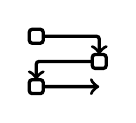
\begin{tikzpicture}[y=0.80pt, x=0.80pt, yscale=-0.800000, xscale=0.800000, inner sep=0pt, outer sep=0pt, rounded corners=1]
\begin{scope}[shift={(8,8)}]
	\node[rectangle, draw=black, line width=1.2, minimum width=5, minimum height=5] (X) at (0cm,0cm) {};
	\node[rectangle, draw=black, line width=1.2, minimum width=5, minimum height=5] (Y) at (1cm,.4cm) {};
	\node[rectangle, draw=black, line width=1.2, minimum width=5, minimum height=5] (Z) at (0cm,.8cm) {};
	\draw[->, line width=1.2] (X) -| (Y);
	\draw[->, line width=1.2] (Y) -| (Z);
	\draw[->, line width=1.2] (Z) -- (1cm,.8cm);
\end{scope}
\end{tikzpicture}
}
\newcommand{\PARDIAGRAMS}{
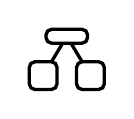
\begin{tikzpicture}[y=0.80pt, x=0.80pt, yscale=-1.000000, xscale=1.000000, inner sep=0pt, outer sep=0pt, rounded corners=2]
\begin{scope}[shift={(8,8)}]
	\node[rectangle, draw=black, line width=1.2, minimum width=15, minimum height=5] (X) at (.5cm,.3cm) {};
	\node[rectangle, draw=black, line width=1.2, minimum width=10, minimum height=10] (Y) at (.2cm,.8cm) {};
	\node[rectangle, draw=black, line width=1.2, minimum width=10, minimum height=10] (Z) at (.8cm,.8cm) {};
	\draw[line width=1.2] (X) -- (Y);
	\draw[line width=1.2] (X) -- (Z);
\end{scope}
\end{tikzpicture}
}
\newcommand{\PARVARIABLES}{
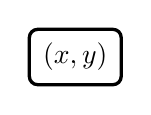
\begin{tikzpicture}[y=0.80pt, x=0.80pt, yscale=-1.000000, xscale=1.000000, inner sep=0pt, outer sep=0pt]
\begin{scope}[shift={(8,8)}]
	\node[rectangle, draw=black, line width=1.2, minimum width=15, minimum height=5, inner sep=5, rounded corners=3] (X) at (.5cm,.5cm) {$(x,y)$};
\end{scope}
\end{tikzpicture}
}
\newcommand{\PARPRONOUNS}{
	\raisebox{-.9cm}[0cm][0cm]{
		\makebox[1cm]{

\begin{tikzpicture}[y=0.80pt, x=0.80pt, yscale=-1.000000, xscale=1.000000, inner sep=0pt, outer sep=0pt]
\begin{scope}[shift={(8,8)}]
	\node[rotate=30, anchor=west] (X) at (.5cm,.5cm) {\begin{tabular}{c}{\sf That} \\ {\sf It}\end{tabular}};
\end{scope}
\end{tikzpicture}
}}}
\newcommand{\PARCALCULATIONS}{
	\raisebox{-.74cm}[0cm][0cm]{
		\makebox[1cm]{
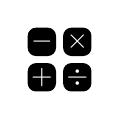
\begin{tikzpicture}[y=0.80pt, x=0.80pt, yscale=-0.900000, xscale=0.900000, inner sep=0pt, outer sep=0pt, rounded corners=3]
\begin{scope}[shift={(8,8)}]
	\fill (0.05cm,0.05cm) rectangle (0.45cm,0.45cm);
    \fill (0.05cm,0.55cm) rectangle (0.45cm,0.95cm);
    \fill (0.55cm,0.05cm) rectangle (0.95cm,0.45cm);
    \fill (0.55cm,0.55cm) rectangle (0.95cm,0.95cm);
    \node[white] at (.25cm, .25cm) {$\pmb{-}$};
	\node[white] at (.75cm, .25cm) {$\pmb{\times}$};
	\node[white] at (.25cm, .75cm) {$\pmb{+}$};
	\node[white] at (.75cm, .75cm) {$\pmb{\div}$};
\end{scope}
\end{tikzpicture}
%\begin{tikzpicture}[y=0.80pt, x=0.80pt, yscale=-1.000000, xscale=1.000000, inner sep=0pt, outer sep=0pt,rounded corners=2]
%\begin{scope}[shift={(8,8)}]
%	\node[] at (.25cm, .25cm) {$-$};
%	\node[] at (.75cm, .25cm) {$\times$};
%	\node[] at (.25cm, .75cm) {$+$};
%	\node[] at (.75cm, .75cm) {$\div$};
%\end{scope}
%\end{tikzpicture}
}}
}
\newcommand{\PAREXPLAIN}{
	\raisebox{-.45cm}[0cm][0cm]{
		\makebox[1cm]{

\begin{tikzpicture}[y=0.80pt, x=0.80pt, yscale=-0.800000, xscale=0.800000, inner sep=0pt, outer sep=0pt]
\begin{scope}[shift={(0,-999.21265)}]
  \path[draw=black,line join=round,line cap=round,miter limit=4.00,line    width=1.200pt] (25.5530,1037.8286)arc(94.842:180.403:19.695244 and    15.909)arc(180.403:265.964:19.695244 and 15.909)arc(265.964:351.525:19.695244    and 15.909)arc(-8.475:77.086:19.695244 and 15.909);
  \path[draw=black,line join=round,line cap=round,miter limit=4.00,even odd    rule,line width=1.200pt] (31.2763,1037.8962) .. controls (27.8741,1042.0646)    and (25.9284,1043.3789) .. (21.3505,1044.5764) .. controls (25.0988,1041.3274)    and (25.5667,1037.9753) .. (25.5667,1037.9753);
  \end{scope}
    \node[text=black] at (28,23) {\small \sf Why?};
\end{tikzpicture}
}}
}
\newcommand{\PARDEFINITIONS}{
	\raisebox{-.475cm}[0cm][0cm]{
		\makebox[1cm]{

\begin{tikzpicture}[y=0.80pt, x=0.80pt, yscale=-0.7000000, xscale=0.700000, inner sep=0pt, outer sep=0pt]
\begin{scope}[shift={(0,-1010)}]
  \path[draw=black,line join=round,line cap=round,miter limit=4.00,even odd    rule,line width=2.400pt] (48.3171,1013.5274) -- (48.3171,1047.0864) --    (9.4043,1047.0864) .. controls (7.7605,1046.5517) and (6.3568,1045.7401) ..    (6.0181,1043.7002) -- (6.0181,1007.0251) .. controls (6.3521,1005.1524) and    (7.4252,1004.1176) .. (9.1836,1003.8596) -- (43.0907,1003.8596) --    (43.0907,1038.7065) -- (9.6678,1038.7065) .. controls (7.1278,1039.1549) and    (6.1084,1040.4467) .. (6.0840,1042.2904);
  \path[fill=black,line join=round,line cap=round,miter limit=4.00,line    width=2.400pt,rounded corners=0.0000cm] (7.1918,1004.5908) rectangle    (42.9425,1038.5253);
\end{scope}
%    \node[text=white] at (25,15) {\Large \bf Aa};
\end{tikzpicture}
}}
}
\newcommand{\PARSETUP}{
	\raisebox{-.475cm}[0cm][0cm]{
		\makebox[1cm]{

\begin{tikzpicture}[y=0.80pt, x=0.80pt, yscale=-0.700000, xscale=0.700000, inner sep=0pt, outer sep=0pt]
\begin{scope}[shift={(0,-999.21265)}]
  \path[draw=white,fill=black,line join=miter,line cap=butt,miter
    limit=4.00,even odd rule,line width=0.250pt] (14.4931,1004.7869) .. controls    (14.4931,1004.7869) and (14.1167,1004.2210) .. (14.0821,1002.8922) .. controls    (14.5853,1002.5912) and (15.1067,1002.3217) .. (15.6434,1002.0854) .. controls    (16.7072,1002.8824) and (16.9511,1003.5168) .. (16.9511,1003.5168) --    (17.5626,1005.1197) .. controls (18.3032,1004.8372) and (19.0731,1004.6385) ..    (19.8579,1004.5274) -- (19.6175,1002.8288) .. controls (19.6175,1002.8288) and    (19.5239,1002.1556) .. (20.0693,1000.9433) .. controls (20.6533,1000.8903) and    (21.2400,1000.8743) .. (21.8261,1000.8943) .. controls (22.4387,1002.0740) and    (22.3832,1002.7514) .. (22.3832,1002.7514) -- (22.2387,1004.4608) .. controls    (23.0285,1004.5278) and (23.8084,1004.6827) .. (24.5637,1004.9231) --    (25.0841,1003.2884) .. controls (25.0841,1003.2884) and (25.2919,1002.6413) ..    (26.3092,1001.7857) .. controls (26.8583,1001.9914) and (27.3941,1002.2311) ..    (27.9134,1002.5034) .. controls (27.9536,1003.8321) and (27.6096,1004.4182) ..    (27.6096,1004.4182) -- (26.7377,1005.8957) .. controls (27.4204,1006.2986) and    (28.0557,1006.7766) .. (28.6319,1007.3210) -- (29.8101,1006.0740) .. controls    (29.8101,1006.0740) and (30.2780,1005.5811) .. (31.5659,1005.2516) .. controls    (31.9713,1005.6753) and (32.3500,1006.1237) .. (32.6998,1006.5943) .. controls    (32.1595,1007.8088) and (31.5953,1008.1877) .. (31.5953,1008.1877) --    (30.1687,1009.1406) .. controls (30.6089,1009.7997) and (30.9739,1010.5061) ..    (31.2569,1011.2466) -- (32.8594,1010.6342) .. controls (32.8594,1010.6342) and    (33.4949,1010.3932) .. (34.7981,1010.6552) .. controls (34.9796,1011.2128) and    (35.1263,1011.7811) .. (35.2372,1012.3569) .. controls (34.2234,1013.2168) and    (33.5507,1013.3133) .. (33.5507,1013.3133) -- (31.8519,1013.5528) .. controls    (31.9626,1014.3377) and (31.9850,1015.1325) .. (31.9186,1015.9224) --    (33.6282,1016.0660) .. controls (33.6282,1016.0660) and (34.3053,1016.1250) ..    (35.3658,1016.9260) .. controls (35.2874,1017.5071) and (35.1729,1018.0828) ..    (35.0231,1018.6497) .. controls (33.7366,1018.9845) and (33.0886,1018.7796) ..    (33.0886,1018.7796) -- (31.4542,1018.2584) .. controls (31.2133,1019.0135) and    (30.8886,1019.7393) .. (30.4861,1020.4222) -- (31.9641,1021.2933) .. controls    (31.9641,1021.2933) and (32.5487,1021.6399) .. (33.1565,1022.8221) .. controls    (32.8337,1023.3117) and (32.4808,1023.7807) .. (32.0998,1024.2264) .. controls    (30.7955,1023.9699) and (30.3005,1023.5041) .. (30.3005,1023.5041) --    (29.0541,1022.3253) .. controls (28.5095,1022.9012) and (27.9020,1023.4143) ..    (27.2431,1023.8549) -- (28.1967,1025.2810) .. controls (28.1967,1025.2810) and    (28.5731,1025.8469) .. (28.6077,1027.1757) .. controls (28.1045,1027.4767) and    (27.5830,1027.7462) .. (27.0464,1027.9825) .. controls (25.9825,1027.1855) and    (25.7387,1026.5511) .. (25.7387,1026.5511) -- (25.1272,1024.9482) .. controls    (24.3866,1025.2307) and (23.6167,1025.4294) .. (22.8318,1025.5405) --    (23.0722,1027.2391) .. controls (23.0722,1027.2391) and (23.1658,1027.9123) ..    (22.6204,1029.1246) .. controls (22.0364,1029.1776) and (21.4497,1029.1936) ..    (20.8637,1029.1736) .. controls (20.2510,1027.9939) and (20.3066,1027.3165) ..    (20.3066,1027.3165) -- (20.4511,1025.6071) .. controls (19.6612,1025.5401) and    (18.8814,1025.3852) .. (18.1261,1025.1448) -- (17.6057,1026.7795) .. controls    (17.6057,1026.7795) and (17.3979,1027.4266) .. (16.3805,1028.2822) .. controls    (15.8314,1028.0765) and (15.2957,1027.8368) .. (14.7763,1027.5645) .. controls    (14.7362,1026.2358) and (15.0801,1025.6497) .. (15.0801,1025.6497) --    (15.9520,1024.1722) .. controls (15.2694,1023.7693) and (14.6340,1023.2913) ..    (14.0578,1022.7469) -- (12.8797,1023.9939) .. controls (12.8797,1023.9939) and    (12.4117,1024.4868) .. (11.1239,1024.8163) .. controls (10.7184,1024.3926) and    (10.3397,1023.9442) .. (9.9899,1023.4736) .. controls (10.5302,1022.2591) and    (11.0945,1021.8802) .. (11.0945,1021.8802) -- (12.5211,1020.9273) .. controls    (12.0808,1020.2682) and (11.7158,1019.5618) .. (11.4329,1018.8213) --    (9.8303,1019.4337) .. controls (9.8303,1019.4337) and (9.1949,1019.6747) ..    (7.8916,1019.4127) .. controls (7.7101,1018.8551) and (7.5635,1018.2868) ..    (7.4525,1017.7110) .. controls (8.4663,1016.8511) and (9.1390,1016.7546) ..    (9.1390,1016.7546) -- (10.8378,1016.5151) .. controls (10.7272,1015.7302) and    (10.7048,1014.9354) .. (10.7711,1014.1455) -- (9.0616,1014.0019) .. controls    (9.0616,1014.0019) and (8.3845,1013.9429) .. (7.3240,1013.1419) .. controls    (7.4024,1012.5608) and (7.5168,1011.9851) .. (7.6667,1011.4182) .. controls    (8.9531,1011.0834) and (9.6011,1011.2883) .. (9.6011,1011.2883) --    (11.2356,1011.8095) .. controls (11.4764,1011.0544) and (11.8011,1010.3286) ..    (12.2036,1009.6457) -- (10.7257,1008.7746) .. controls (10.7257,1008.7746) and    (10.1410,1008.4280) .. (9.5333,1007.2458) .. controls (9.8561,1006.7562) and    (10.2090,1006.2872) .. (10.5900,1005.8415) .. controls (11.8943,1006.0980) and    (12.3892,1006.5638) .. (12.3892,1006.5638) -- (13.6356,1007.7426) .. controls    (14.1803,1007.1667) and (14.7878,1006.6536) .. (15.4467,1006.2130) --    (14.4931,1004.7869)(32.4345,1021.7376) .. controls (32.4345,1021.7376) and    (32.0553,1021.1433) .. (32.1914,1019.7860) .. controls (32.6707,1019.5290) and    (33.1690,1019.3092) .. (33.6820,1019.1286) .. controls (34.7760,1019.9434) and    (34.9592,1020.6241) .. (34.9592,1020.6241) -- (35.4008,1022.2975) .. controls    (36.1173,1022.1084) and (36.8591,1022.0331) .. (37.5990,1022.0742) --    (37.6952,1020.3462) .. controls (37.6952,1020.3462) and (37.7378,1019.6426) ..    (38.6456,1018.6244) .. controls (39.1844,1018.6984) and (39.7168,1018.8133) ..    (40.2380,1018.9687) .. controls (40.6441,1020.2710) and (40.3922,1020.9294) ..    (40.3922,1020.9294) -- (39.7659,1022.5428) .. controls (40.4567,1022.8109) and    (41.1011,1023.1860) .. (41.6755,1023.6542) -- (42.7690,1022.3127) .. controls    (42.7690,1022.3127) and (43.2171,1021.7685) .. (44.5500,1021.4784) .. controls    (44.9425,1021.8548) and (45.3055,1022.2609) .. (45.6358,1022.6929) .. controls    (45.1990,1023.9852) and (44.6082,1024.3698) .. (44.6082,1024.3698) --    (43.1532,1025.3069) .. controls (43.5544,1025.9299) and (43.8553,1026.6121) ..    (44.0448,1027.3285) -- (45.7179,1026.8860) .. controls (45.7179,1026.8860) and    (46.4003,1026.7091) .. (47.6492,1027.2579) .. controls (47.7455,1027.7931) and    (47.8005,1028.3350) .. (47.8138,1028.8787) .. controls (46.7008,1029.6673) and    (45.9968,1029.6312) .. (45.9968,1029.6312) -- (44.2688,1029.5342) .. controls    (44.2272,1030.2741) and (44.0696,1031.0029) .. (43.8018,1031.6939) --    (45.4156,1032.3193) .. controls (45.4156,1032.3193) and (46.0716,1032.5772) ..    (46.7594,1033.7553) .. controls (46.5227,1034.2449) and (46.2487,1034.7156) ..    (45.9399,1035.1633) .. controls (44.5759,1035.1473) and (44.0276,1034.7041) ..    (44.0276,1034.7041) -- (42.6867,1033.6099) .. controls (42.2181,1034.1840) and    (41.6623,1034.6810) .. (41.0395,1035.0826) -- (41.9774,1036.5371) .. controls    (41.9774,1036.5371) and (42.3565,1037.1314) .. (42.2205,1038.4887) .. controls    (41.7412,1038.7457) and (41.2429,1038.9655) .. (40.7299,1039.1461) .. controls    (39.6359,1038.3313) and (39.4527,1037.6506) .. (39.4527,1037.6506) --    (39.0111,1035.9772) .. controls (38.2946,1036.1663) and (37.5528,1036.2416) ..    (36.8129,1036.2005) -- (36.7167,1037.9285) .. controls (36.7167,1037.9285) and    (36.6741,1038.6321) .. (35.7663,1039.6503) .. controls (35.2274,1039.5763) and    (34.6951,1039.4614) .. (34.1739,1039.3060) .. controls (33.7678,1038.0037) and    (34.0197,1037.3453) .. (34.0197,1037.3453) -- (34.6460,1035.7319) .. controls    (33.9552,1035.4638) and (33.3108,1035.0887) .. (32.7364,1034.6205) --    (31.6429,1035.9620) .. controls (31.6429,1035.9620) and (31.1948,1036.5062) ..    (29.8619,1036.7963) .. controls (29.4694,1036.4199) and (29.1063,1036.0138) ..    (28.7761,1035.5818) .. controls (29.2129,1034.2895) and (29.8037,1033.9049) ..    (29.8037,1033.9049) -- (31.2587,1032.9678) .. controls (30.8575,1032.3448) and    (30.5566,1031.6626) .. (30.3671,1030.9462) -- (28.6940,1031.3887) .. controls    (28.6940,1031.3887) and (28.0116,1031.5656) .. (26.7627,1031.0168) .. controls    (26.6664,1030.4816) and (26.6114,1029.9397) .. (26.5981,1029.3960) .. controls    (27.7111,1028.6074) and (28.4151,1028.6435) .. (28.4151,1028.6435) --    (30.1431,1028.7405) .. controls (30.1847,1028.0006) and (30.3422,1027.2718) ..    (30.6101,1026.5808) -- (28.9963,1025.9554) .. controls (28.9963,1025.9554) and    (28.3403,1025.6975) .. (27.6525,1024.5194) .. controls (27.8892,1024.0298) and    (28.1632,1023.5591) .. (28.4720,1023.1114) .. controls (29.8360,1023.1274) and    (30.3843,1023.5706) .. (30.3843,1023.5706) -- (31.7252,1024.6648) .. controls    (32.1938,1024.0907) and (32.7496,1023.5937) .. (33.3724,1023.1921) --    (32.4345,1021.7376)(31.3692,1036.2205) .. controls (31.3692,1036.2205) and    (31.9636,1035.7958) .. (33.3506,1035.9783) .. controls (33.6046,1036.4235) and    (33.8193,1036.8899) .. (33.9924,1037.3723) .. controls (33.2292,1038.5448) and    (32.5201,1038.7203) .. (32.5201,1038.7203) -- (30.8296,1039.1248) .. controls    (30.9915,1039.8014) and (31.0188,1040.5034) .. (30.9098,1041.1906) --    (32.6266,1041.4629) .. controls (32.6266,1041.4629) and (33.3471,1041.5829) ..    (34.1989,1042.6927) .. controls (34.0636,1043.1871) and (33.8857,1043.6687) ..    (33.6670,1044.1322) .. controls (32.2982,1044.4216) and (31.6728,1044.0442) ..    (31.6728,1044.0442) -- (30.1914,1043.1348) .. controls (29.8274,1043.7278) and    (29.3503,1044.2434) .. (28.7873,1044.6522) -- (29.8087,1046.0587) .. controls    (29.8087,1046.0587) and (30.2333,1046.6531) .. (30.0508,1048.0402) .. controls    (29.6057,1048.2941) and (29.1393,1048.5088) .. (28.6569,1048.6820) .. controls    (27.4844,1047.9187) and (27.3089,1047.2097) .. (27.3089,1047.2097) --    (26.9044,1045.5191) .. controls (26.2277,1045.6810) and (25.5258,1045.7083) ..    (24.8386,1045.5991) -- (24.5663,1047.3159) .. controls (24.5663,1047.3159) and    (24.4463,1048.0364) .. (23.3365,1048.8882) .. controls (22.8421,1048.7529) and    (22.3605,1048.5750) .. (21.8970,1048.3563) .. controls (21.6076,1046.9876) and    (21.9849,1046.3621) .. (21.9849,1046.3621) -- (22.8942,1044.8807) .. controls    (22.3013,1044.5167) and (21.7857,1044.0396) .. (21.3768,1043.4766) --    (19.9703,1044.4980) .. controls (19.9703,1044.4980) and (19.3760,1044.9227) ..    (17.9889,1044.7402) .. controls (17.7350,1044.2950) and (17.5202,1043.8286) ..    (17.3471,1043.3462) .. controls (18.1103,1042.1737) and (18.8194,1041.9982) ..    (18.8194,1041.9982) -- (20.5099,1041.5937) .. controls (20.3480,1040.9171) and    (20.3208,1040.2151) .. (20.4298,1039.5279) -- (18.7130,1039.2556) .. controls    (18.7130,1039.2556) and (17.9925,1039.1356) .. (17.1407,1038.0258) .. controls    (17.2759,1037.5314) and (17.4539,1037.0498) .. (17.6726,1036.5863) .. controls    (19.0413,1036.2969) and (19.6668,1036.6743) .. (19.6668,1036.6743) --    (21.1482,1037.5837) .. controls (21.5122,1036.9907) and (21.9893,1036.4751) ..    (22.5523,1036.0663) -- (21.5309,1034.6598) .. controls (21.5309,1034.6598) and    (21.1062,1034.0654) .. (21.2887,1032.6783) .. controls (21.7339,1032.4244) and    (22.2003,1032.2097) .. (22.6827,1032.0365) .. controls (23.8552,1032.7998) and    (24.0306,1033.5088) .. (24.0306,1033.5088) -- (24.4351,1035.1994) .. controls    (25.1118,1035.0375) and (25.8137,1035.0102) .. (26.5009,1035.1194) --    (26.7732,1033.4026) .. controls (26.7732,1033.4026) and (26.8932,1032.6821) ..    (28.0031,1031.8303) .. controls (28.4974,1031.9656) and (28.9791,1032.1435) ..    (29.4426,1032.3622) .. controls (29.7320,1033.7309) and (29.3547,1034.3564) ..    (29.3547,1034.3564) -- (28.4453,1035.8378) .. controls (29.0383,1036.2018) and    (29.5539,1036.6789) .. (29.9627,1037.2419) -- (31.3692,1036.2205);  
  \path[fill=white,line join=round,line cap=round,miter limit=4.00,line width=0.240pt] (21.3511,1014.9621) circle (0.2027cm);
  \path[fill=white,line join=round,line cap=round,miter limit=4.00,line width=0.240pt] (37.2980,1029.0370) circle (0.1288cm);
  \path[fill=white,line join=round,line cap=round,miter limit=4.00,line width=0.240pt] (25.6774,1040.4004) circle (0.0841cm);
\end{scope}
\end{tikzpicture}
}}
}
\newcommand{\PARCHECK}{
	\raisebox{-.46cm}[0cm][0cm]{
		\makebox[1cm]{

\begin{tikzpicture}[y=0.80pt, x=0.80pt, yscale=-0.70000, xscale=0.70000, inner sep=0pt, outer sep=0pt]
\begin{scope}[shift={(0,-999.21265)}]
  \path[shift={(0,999.21265)},color=black,fill=black,line join=round,line    cap=butt,miter limit=4.00,nonzero rule,line width=2.400pt] (7.5508,6.9805) ..    controls (5.0037,6.9805) and (2.9062,9.0779) .. (2.9062,11.6250) --    (2.9062,46.1855) .. controls (2.9062,48.7326) and (5.0037,50.8301) ..    (7.5508,50.8301) -- (42.1113,50.8301) .. controls (44.6584,50.8301) and    (46.7559,48.7326) .. (46.7559,46.1855) -- (46.7559,18.0312) --    (43.7559,21.0312) -- (43.7559,46.1855) .. controls (43.7559,47.1225) and    (43.0483,47.8301) .. (42.1113,47.8301) -- (7.5508,47.8301) .. controls    (6.6138,47.8301) and (5.9062,47.1225) .. (5.9062,46.1855) -- (5.9062,11.6250)    .. controls (5.9062,10.6880) and (6.6138,9.9805) .. (7.5508,9.9805) --    (32.9551,9.9805) -- (35.9551,6.9805) -- (7.5508,6.9805) -- cycle;
  \path[draw=black,line join=round,line cap=round,miter limit=4.00,even odd rule,line width=4.400pt] (46.8750,1006.3801) -- (24.2411,1028.4783) -- (13.9286,1018.1658);
\end{scope}
\end{tikzpicture}
}}
}
\newcommand{\PARMULTIPLE}{
	\raisebox{-.475cm}[0cm][0cm]{
		\makebox[1cm]{

\begin{tikzpicture}[y=0.80pt, x=0.80pt, yscale=-0.700000, xscale=0.700000, inner sep=0pt, outer sep=0pt]
\begin{scope}[shift={(0,-999.21265)}]
  \begin{scope}[cm={{1.06005,0.0,0.0,1.06005,(-0.43529,-63.0815)}},fill=black]
    \path[fill=black,miter limit=4.00,line width=2.400pt,rounded corners=0.0000cm]      (21.7857,1016.0230) rectangle (29.2857,1050.4873);
    \path[cm={{1.31936,0.0,0.0,1.0,(-7.52516,0.0)}},fill=black,miter limit=4.00,line      width=2.400pt] (32.7892,1018.0207) -- (17.1329,1017.8859) --      (25.0778,1004.3946) -- cycle;
  \end{scope}
  \begin{scope}[cm={{0.38993,-0.38993,0.38993,0.38993,(-394.3635,647.0653)}}]
    \path[fill=black,miter limit=4.00,line width=2.400pt,rounded corners=0.0000cm]      (21.7857,1016.0230) rectangle (29.2857,1050.4873);
    \path[cm={{1.31936,0.0,0.0,1.0,(-7.52516,0.0)}},fill=black,miter limit=4.00,line      width=2.400pt] (32.7892,1018.0207) -- (17.1329,1017.8859) --      (25.0778,1004.3946) -- cycle;
  \end{scope}
  \begin{scope}[cm={{0.38993,0.38993,-0.38993,0.38993,(427.78629,627.0836)}}]
    \path[fill=black,miter limit=4.00,line width=2.400pt,rounded corners=0.0000cm]      (21.7857,1016.0230) rectangle (29.2857,1050.4873);
    \path[cm={{1.31936,0.0,0.0,1.0,(-7.52516,0.0)}},fill=black,miter limit=4.00,line      width=2.400pt] (32.7892,1018.0207) -- (17.1329,1017.8859) --      (25.0778,1004.3946) -- cycle;
  \end{scope}
\end{scope}
\end{tikzpicture}
}}
}
\newcommand{\PAROTHER}{

\begin{tikzpicture}[y=0.80pt, x=0.80pt, yscale=.5000000, xscale=.500000, inner sep=0pt, outer sep=0pt]
\begin{scope}[shift={(0,-1016.9292)}]
  \path[draw=black,line join=round,line cap=round,miter limit=4.00,line width=1.200pt] (26.6071,1035.0406) circle (0.1768cm);
  \path[draw=black,line join=round,line cap=round,miter limit=4.00,line width=1.200pt] (9.0714,1035.0229) circle (0.1768cm);
  \path[draw=black,line join=round,line cap=round,miter limit=4.00,line width=1.200pt] (43.9643,1035.1301) circle (0.1768cm);
\end{scope}
\end{tikzpicture}
}

%%%%%%%%%%%%%%%%%%%%%%%%%%%%%%%%%%%%%%%%%%%%%%%%%%%%
% End of the tikz macros for drawing the icons     %
%%%%%%%%%%%%%%%%%%%%%%%%%%%%%%%%%%%%%%%%%%%%%%%%%%%%


	\emph{Due: Sep 19 (draft), Sep 21 (final)} 
		\hspace{1cm} \emph{Name:} \\ %\underline{\hspace{2in}} \\
	\vspace{-0.3cm}
	\hrule
	\par
	
	\begin{centering}
	\emph{The PAR Process}
	\par
	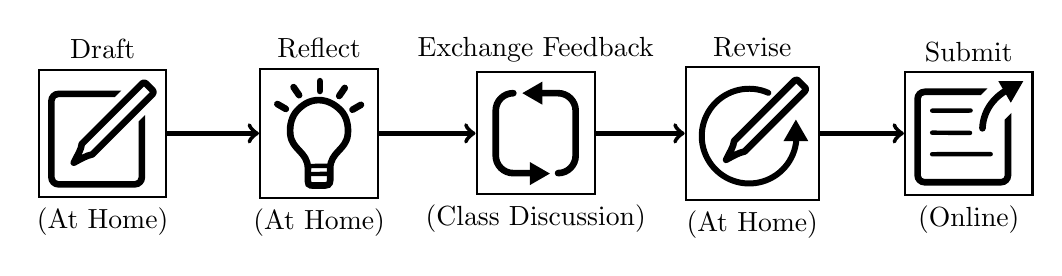
\begin{tikzpicture}
		\def\spacing{2.75}

		\PARPROCESSNODE{A}{\PARDRAFT}{(At Home)}{Draft}{(0,0)}
		\PARPROCESSNODE{B}{\PARREFLECT}{(At Home)}{Reflect}{(\spacing,0)}
		\PARPROCESSNODE{C}{\PAREXCHANGE}{(Class Discussion)}{Exchange Feedback}{(2*\spacing,0)}
		\PARPROCESSNODE{D}{\PARREVISE}{(At Home)}{Revise}{(3*\spacing,0)}
		\PARPROCESSNODE{E}{\PARSUBMIT}{(Online)}{Submit}{(4*\spacing,0)}
		\draw[->, ultra thick] (A) edge (B);
		\draw[->, ultra thick] (B) edge (C);
		\draw[->, ultra thick] (C) edge (D);
		\draw[->, ultra thick] (D) edge (E);
	\end{tikzpicture}
	\end{centering}
	
	\textit{Note: Your PAR (both initial and final drafts) must be typed.}% in \LaTeX.}

	\begin{center}
	\emph{Problem Statement}
	\end{center}
	
You are hired by theBigCompany to help with their ``elevator problem''.

This is the email you received:

\begin{center}
\begin{minipage}{.75\textwidth}
	\email
\end{minipage}
\end{center}

Model the current situation at theBigCompany and write a \emph{one-page} report to the CEO about it.
		
	\bigskip
		
	


	\vfill\par
	\begin{center}
		\emph{Reflection}\\
		Turn the page and check off the icons for things you think you did well; circle the icons for things
		you would like feedback on.
	\end{center}



\newpage
%\newgeometry{total={7in, 10.5in}}

	\pagestyle{empty}
	\hfill\emph{Feedback Provided By:}\underline{\hspace{2in}}\vspace{.2cm}\\
	\begin{minipage}{4cm}\emph{Suggestions}\hfill\end{minipage}\hfill{Communication}\hfill\begin{minipage}{4cm}\hfill\emph{Strengths}\end{minipage}\\
	\vspace{-.3cm}
	\hrule

	\vspace{-.3cm}
	\begin{center}
	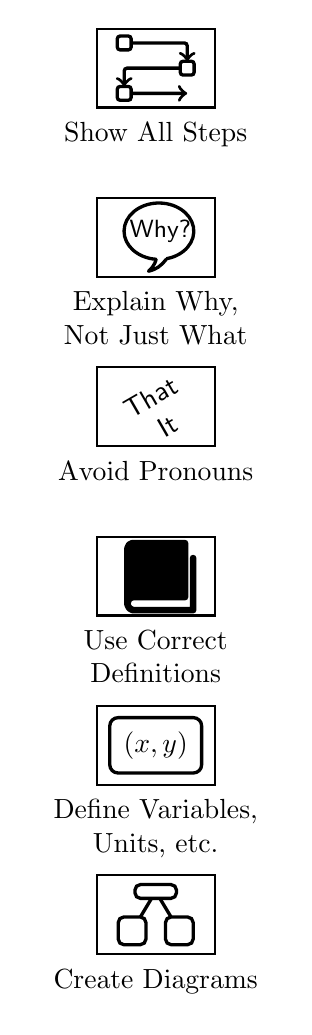
\begin{tikzpicture}
		\def\spacing{2.15cm}
		\PARCHECKLISTNODE{A}{(0,0)}{\PARSTEPS}{Show All Steps}
		\PARCHECKLISTNODE{B}{(0,-1*\spacing)}{\PAREXPLAIN}{Explain Why,\\Not Just What}
		\PARCHECKLISTNODE{C}{(0,-2*\spacing)}{\PARPRONOUNS}{Avoid Pronouns}
		\PARCHECKLISTNODE{D}{(0,-3*\spacing)}{\PARDEFINITIONS}{Use Correct \\Definitions}
		\PARCHECKLISTNODE{E}{(0,-4*\spacing)}{\PARVARIABLES}{Define Variables, \\Units, etc.}
		\PARCHECKLISTNODE{F}{(0,-5*\spacing)}{\PARDIAGRAMS}{Create Diagrams}
	\end{tikzpicture}
	\end{center}
	
	\begin{minipage}{4cm}\emph{Suggestions}\hfill\end{minipage}\hfill{Accuracy}\hfill\begin{minipage}{4cm}\hfill\emph{Strengths}\end{minipage}\\
	\vspace{-.3cm}
	\hrule
	
	\vspace{-0.3cm}
	\begin{center}
	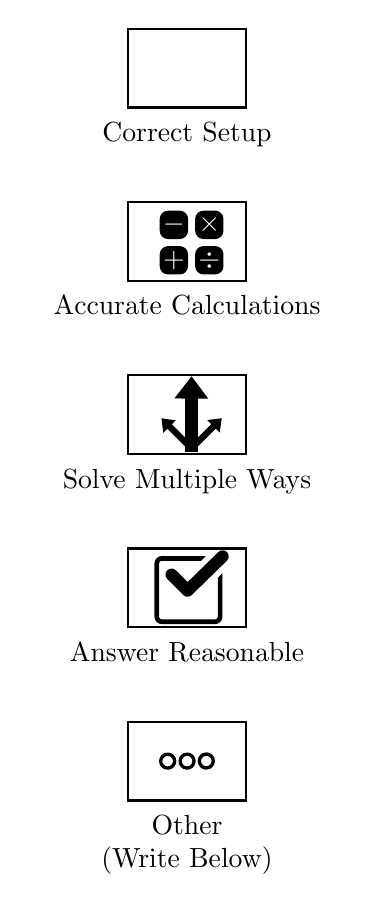
\begin{tikzpicture}
		\def\spacing{2.2cm}
		\PARCHECKLISTNODE{A}{(0,0)}{\PARSETUP}{Correct Setup}
		\PARCHECKLISTNODE{B}{(0,-1*\spacing)}{\PARCALCULATIONS}{Accurate Calculations}
		\PARCHECKLISTNODE{C}{(0,-2*\spacing)}{\PARMULTIPLE}{Solve Multiple Ways}
		\PARCHECKLISTNODE{D}{(0,-3*\spacing)}{\PARCHECK}{Answer Reasonable}
		\PARCHECKLISTNODE{E}{(0,-4*\spacing)}{\PAROTHER}{Other \\(Write Below)}
	\end{tikzpicture}
	\end{center}


%\restoregeometry


	
%\end{instructoronly}
\end{lesson}





%\newpage

%\question
%Another question to be added here
%
%\newpage





%
%
%
%
%\begin{module}
%	\Title{Putting it all together}
%	\Heading{Textbook} \href{https://m3challenge.siam.org/resources/modeling-handbook}{Math Modelling: Getting started and getting solutions, Bliss-Fowler-Galluzzo}
%	
%	\Heading{Objectives}
%	\begin{itemize}
%		\item Bla bla bla	
%	\end{itemize}
%	
%	\Heading{Motivation} 
%
%
%\end{module}
%
%
%
%
%\section*{Step F. Writing a report}\label{F-report}
%\addcontentsline{toc}{subsection}{Step F. Writing a report}
%


